\section{Le marché concurrentiel}

This chapter is the course's account of the \textbf{marché concurrentiel}
(\textit{competitive market}), in three steps: demand, supply, and the
équilibre de marché at which they meet. Demand comes first and takes the most room. The
demande individuelle of one consumer is explained by their choice between two goods,
drawn with courbes d'indifférence, the taux marginal de substitution and the
contrainte budgétaire; the optimum du consommateur then yields the fonction de
demande. Individual demands add up to the demande agrégée, which can shift, and
whose response to the price is measured by the élasticité de la demande. Supply is
described in the same terms: the courbe d'offre, its élasticité, the factors that
influence it and its déplacements.\\

The équilibre de marché is then put to work. Déplacements de la demande et de
l'offre move it;
a contrôle des prix, by a prix plafond or a prix plancher, holds the price away from
it and leaves a pénurie or an excédent; and a tax opens a gap between the price
buyers pay and the price sellers receive, whose burden the two sides share in
proportions set by their élasticités. Three limits of taxation, only named, close
the chapter.

\subsection{La demande individuelle}

A consumer's \textbf{demande individuelle} (\textit{individual demand}) for a good
can be set out in two ways. The \textbf{barème de demande} (\textit{demand
schedule}) lists, price by price, the \textbf{quantité demandée} (\textit{quantity
demanded}). The \textbf{courbe de demande} (\textit{demand curve}) draws the same
barème de demande as a graph, the quantité demandée of the good against its price.
It slopes downward: the cheaper the good, the larger the quantité demandée.

\begin{figure}[h!]
  \centering
  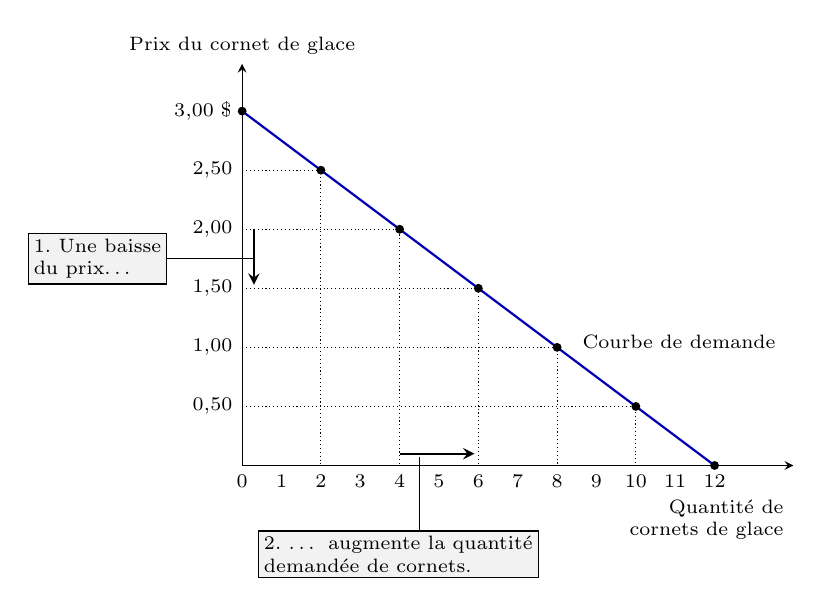
\begin{tikzpicture}[x=0.5cm,y=1.5cm,font=\scriptsize,>=stealth,
      call/.style={draw,fill=black!5,align=left,inner sep=2pt}]
    % axes
    \draw[->] (0,0) -- (14,0);
    \draw[->] (0,0) -- (0,3.4);
    \node[above] at (0,3.4) {Prix du cornet de glace};
    \node[below left,align=right] at (14,-0.21) {Quantité de\\cornets de glace};
    \foreach \q in {0,...,12} \node[below] at (\q,0) {$\q$};
    \foreach \p/\l in {0.5/{$0{,}50$},1/{$1{,}00$},1.5/{$1{,}50$},2/{$2{,}00$},
        2.5/{$2{,}50$},3/{$3{,}00$~\$}}
      \node[left] at (0,\p) {\l};
    % the seven rows of the schedule
    \foreach \k in {0,...,6} {
      \draw[densely dotted] (0,{3-0.5*\k}) -| ({2*\k},0);
    }
    \draw[blue!70!black,thick] (0,3) -- (12,0);
    \foreach \k in {0,...,6} \fill ({2*\k},{3-0.5*\k}) circle (1.6pt);
    \node[right] at (8.4,1.05) {Courbe de demande};
    % a fall in the price raises the quantity demanded
    \draw[->,thick] (0.3,2) -- (0.3,1.53);
    \node[call,anchor=east] (c1) at (-1.9,1.75) {1.\ Une baisse\\du prix\ldots};
    \draw (c1.east) -- (0.3,1.75);
    \draw[->,thick] (4,0.1) -- (5.9,0.1);
    \node[call,anchor=north west] (c2) at (0.4,-0.55)
      {2.\ \ldots{} augmente la quantité\\demandée de cornets.};
    \draw (4.5,-0.55) -- (4.5,0.07);
  \end{tikzpicture}
  \caption*{\small La demande individuelle de Catherine. The barème de demande
  plotted point by point; a lower price raises the quantité demandée, so the
  courbe de demande slopes downward.}
\end{figure}

\begin{example}[Le barème de demande de Catherine]
  Catherine's barème de demande for ice-cream cones:
  \begin{center}
    \begin{tabular}{@{}cc@{}}
      \toprule
      Prix du cornet de glace & Quantité de cornets demandée \\
      \midrule
      $0{,}00$~\$ & 12 cornets \\
      $0{,}50$ & 10 \\
      $1{,}00$ & 8 \\
      $1{,}50$ & 6 \\
      $2{,}00$ & 4 \\
      $2{,}50$ & 2 \\
      $3{,}00$ & 0 \\
      \bottomrule
    \end{tabular}
  \end{center}
  Catherine's courbe de demande plots the seven rows of the table. A fall in the
  price from 2,00 to 1,50~\$ raises the quantité demandée from 4 to 6 cones.
\end{example}

The next figures explain the demande individuelle by the consumer's choice
between two goods, pizza and Pepsi.

\subsubsection{Courbes d'indifférence}

\textbf{Courbes d'indifférence} (\textit{indifference curves}) represent the
consumer's preferences. Each curve joins the baskets of pizza and Pepsi that please
them equally. Since they would rather have more of a good than less, any basket on a
higher courbe d'indifférence beats any basket on a lower one. In the figure, $A$,
$B$ and $C$, all on $I_1$, are worth the same to them, and $D$, on the higher $I_2$,
is better than each of them. The small step drawn at $B$ is the TMS, defined
below.\\

\begin{figure}[h!]
  \centering
  \begin{tikzpicture}[font=\scriptsize,>=stealth]
    \draw[->] (0,0) -- (7.4,0);
    \draw[->] (0,0) -- (0,6.1);
    \node[above] at (0,6.1) {Quantité de Pepsi};
    \node[below left] at (7.4,-0.05) {Quantité de pizzas};
    \node[below left] at (0,0) {$0$};
    \draw[blue!70!black,thick] plot[domain=0.7:6.2,samples=80] (\x,{4/\x});
    \draw[blue!70!black,thick] plot[domain=1.4:6.6,samples=80] (\x,{8/\x});
    \node[right,align=left] at (6.2,0.75) {Courbe\\d'indifférence $I_1$};
    \node[right] at (6.6,1.21) {$I_2$};
    % points
    \fill (1,4) circle (1.6pt) node[above right] {$C$};
    \fill (2,2) circle (1.6pt) node[above right] {$B$};
    \fill (3.5,{4/3.5}) circle (1.6pt) node[below left] {$A$};
    \fill (4,2) circle (1.6pt) node[above right] {$D$};
    % the step at B
    \draw (2,2) -- (2,1.6) -- (2.5,1.6);
    \node[left] at (2,1.8) {TMS};
    \node[below] at (2.25,1.6) {$1$};
  \end{tikzpicture}
  \caption*{\small Les préférences du consommateur. $A$, $B$ and $C$ lie on one
  courbe d'indifférence, $I_1$; $D$, on the higher curve $I_2$, is preferred to
  each of them.}
\end{figure}

Two courbes d'indifférence can never cross. Suppose they did, as in the figure
with crossing curves: $A$ and $B$ lie on one curve, $B$ and $C$ on the other, so
$A$, $B$ and $C$ would all be worth the same to the consumer. Yet $C$ holds more
pizza and more Pepsi than $A$.

\begin{figure}[h!]
  \centering
  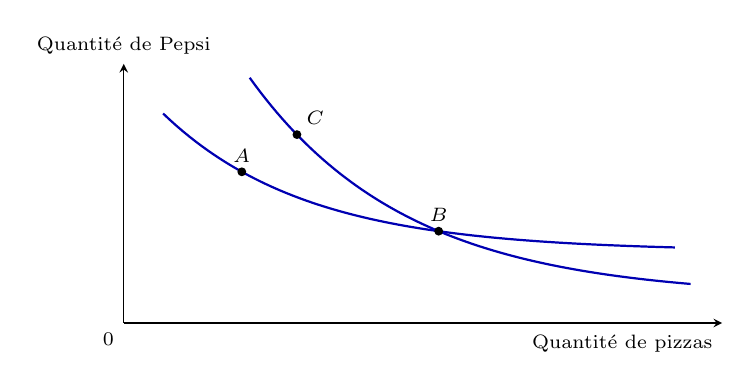
\begin{tikzpicture}[y=0.7cm,font=\scriptsize,>=stealth]
    \draw[->] (0,0) -- (7.6,0);
    \draw[->] (0,0) -- (0,4.7);
    \node[above] at (0,4.7) {Quantité de Pepsi};
    \node[below left] at (7.6,-0.05) {Quantité de pizzas};
    \node[below left] at (0,0) {$0$};
    \draw[blue!70!black,thick] plot[domain=0.5:7,samples=80]
      (\x,{1.3+2.5*exp(-0.55*(\x-0.5))});
    \draw[blue!70!black,thick] plot[domain=1.6:7.2,samples=80]
      (\x,{1.665+1.2*(exp(-0.5*(\x-4))-1)});
    \fill (1.5,2.742) circle (1.6pt) node[above] {$A$};
    \fill (2.2,3.417) circle (1.6pt) node[above right] {$C$};
    \fill (4,1.665) circle (1.6pt) node[above] {$B$};
  \end{tikzpicture}
  \caption*{\small L'impossibilité de courbes d'indifférence sécantes. Such a
  picture is ruled out: it would make $C$ worth no more than $A$, although $C$ holds
  more pizza and more Pepsi.}
\end{figure}

\subsubsection{Taux marginal de substitution}

The \textbf{taux marginal de substitution} (\textit{marginal rate of substitution}),
written TMS, measures how readily the consumer swaps Pepsi for pizza: the amount of
Pepsi they would have to be given to part with one pizza. In the figure of the
consumer's preferences it is the vertical side of the step drawn at $B$, whose
horizontal side is one pizza.\\

Courbes d'indifférence are normally bowed inward, and this shape makes the TMS
depend on how much of each good the consumer already has.

\begin{example}[Le TMS le long d'une courbe d'indifférence]
  At $A$ the consumer has few pizzas and plenty of Pepsi, so only a large amount of
  extra Pepsi would make them give up a pizza: a TMS of 6 pints of Pepsi per pizza.
  Where the position is reversed, as at $B$, with many pizzas and little Pepsi, a
  small amount of extra Pepsi is enough: a TMS of 1 pint of Pepsi per pizza.
\end{example}

\begin{figure}[h!]
  \centering
  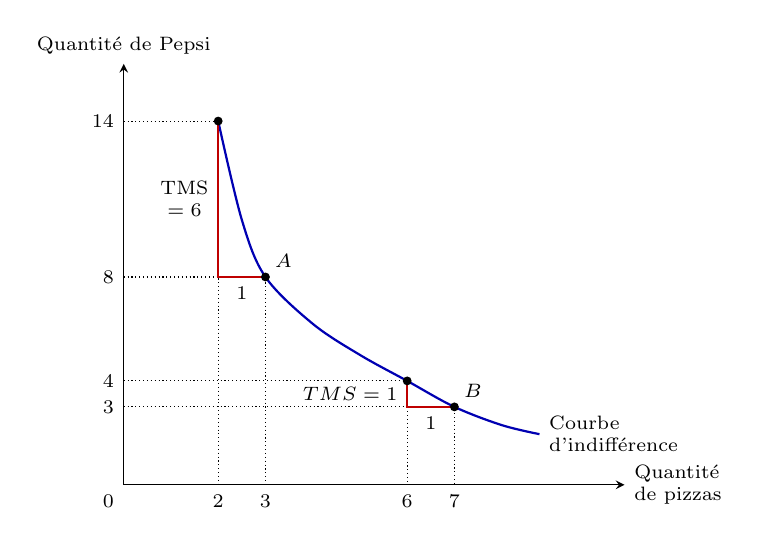
\begin{tikzpicture}[x=0.6cm,y=0.33cm,font=\scriptsize,>=stealth]
    \draw[->] (0,0) -- (10.6,0);
    \draw[->] (0,0) -- (0,16.2);
    \node[above] at (0,16.2) {Quantité de Pepsi};
    \node[right,align=left] at (10.6,0) {Quantité\\de pizzas};
    \node[below left] at (0,0) {$0$};
    % guides and ticks
    \foreach \x/\y in {2/14,3/8,6/4,7/3}
      \draw[densely dotted] (0,\y) -| (\x,0);
    \foreach \x in {2,3,6,7} \node[below] at (\x,0) {$\x$};
    \foreach \y in {3,4,8,14} \node[left] at (0,\y) {$\y$};
    % the courbe d'indifférence
    \draw[blue!70!black,thick] plot[smooth,tension=0.55] coordinates
      {(2,14) (2.5,10.2) (3,8) (4,6.2) (5,5) (6,4) (7,3) (8,2.3) (8.8,1.95)};
    \node[right,align=left] at (8.8,1.95) {Courbe\\d'indifférence};
    % the two steps
    \draw[red!75!black,thick] (2,14) -- (2,8) -- (3,8);
    \draw[red!75!black,thick] (6,4) -- (6,3) -- (7,3);
    \node[left,align=center] at (2,11) {TMS\\$= 6$};
    \node[below] at (2.5,8) {$1$};
    \node[left] at (6,3.5) {$\text{TMS} = 1$};
    \node[below] at (6.5,3) {$1$};
    % points
    \foreach \x/\y in {2/14,3/8,6/4,7/3} \fill (\x,\y) circle (1.6pt);
    \node[above right] at (3,8) {$A$};
    \node[above right] at (7,3) {$B$};
  \end{tikzpicture}
  \caption*{\small Une courbe d'indifférence convexe. To give up one pizza, the
  consumer must be given 6 pints of Pepsi at $A$ but only 1 at $B$: the TMS is
  lower where they have more pizza and less Pepsi.}
\end{figure}

\subsection{L'optimum du consommateur}

\begin{figure}[h!]
  \centering
  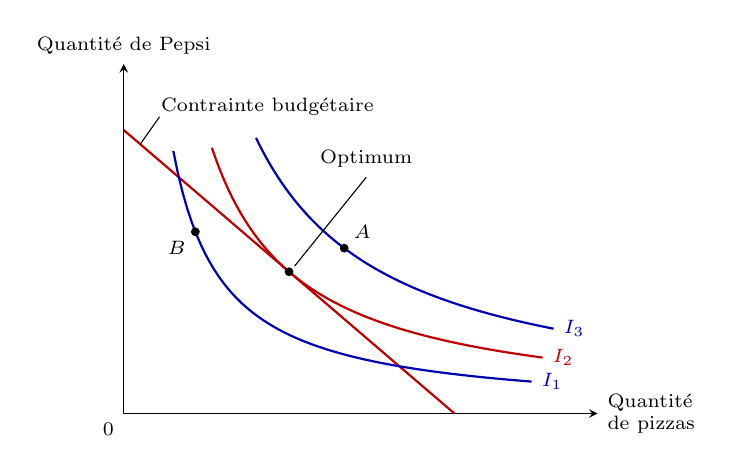
\begin{tikzpicture}[x=0.7cm,y=0.6cm,font=\scriptsize,>=stealth]
    \draw[->] (0,0) -- (8.6,0);
    \draw[->] (0,0) -- (0,7.4);
    \node[above] at (0,7.4) {Quantité de Pepsi};
    \node[right,align=left] at (8.6,0) {Quantité\\de pizzas};
    \node[below left] at (0,0) {$0$};
    % the contrainte budgétaire
    \draw[red!75!black,thick] (0,6) -- (6,0);
    \node[right] at (0.5,6.5) {Contrainte budgétaire};
    \draw (0.65,6.28) -- (0.3,5.7);
    % three courbes d'indifférence
    \draw[blue!70!black,thick] plot[domain=0.9:7.4,samples=80] (\x,{5/\x})
      node[right] {$I_1$};
    \draw[red!75!black,thick] plot[domain=1.6:7.6,samples=80] (\x,{9/\x})
      node[right] {$I_2$};
    \draw[blue!70!black,thick] plot[domain=2.4:7.8,samples=80] (\x,{14/\x})
      node[right] {$I_3$};
    % points
    \fill (3,3) circle (1.6pt);
    \draw (3.1,3.12) -- (4.4,5.0) node[above] {Optimum};
    \fill (4,3.5) circle (1.6pt) node[above right] {$A$};
    \fill (1.3,{5/1.3}) circle (1.6pt) node[below left] {$B$};
  \end{tikzpicture}
  \caption*{\small L'optimum du consommateur. The contrainte budgétaire touches $I_2$
  at the optimum; $A$, on $I_3$, lies beyond the contrainte budgétaire, and $B$,
  below it, lies on the lower $I_1$.}
\end{figure}

The consumer cannot afford every basket of pizza and Pepsi. Their
\textbf{contrainte budgétaire} (\textit{budget constraint}) is drawn as a straight
line: the baskets on it or below it are affordable, those beyond it are not. Of the
baskets on their contrainte budgétaire, they pick the one on the highest courbe
d'indifférence. At this \textbf{optimum du consommateur} (\textit{consumer's
optimum}) the courbe d'indifférence just touches the contrainte budgétaire, and the
TMS equals the \textbf{prix relatif} (\textit{relative price}) of the two goods.\\

In the figure, $I_2$ is the highest courbe d'indifférence within their reach. They would
rather have the basket $A$, on $I_3$, but it lies beyond their contrainte budgétaire.
The basket $B$ is within it, but it sits on the lower $I_1$, so they like it less
than the optimum.

\subsubsection{Les effets de substitution et de revenu}

Three figures follow under this heading: the first changes the consumer's income,
the other two the price of one good.\\

A rise in the consumer's income moves the contrainte budgétaire out, parallel to
itself. If both goods are \textbf{biens normaux} (\textit{normal goods}), the extra
income goes on more of each: the optimum moves from $I_1$ to the higher $I_2$, with
more pizza and more Pepsi.\\

\begin{figure}[h!]
  \centering
  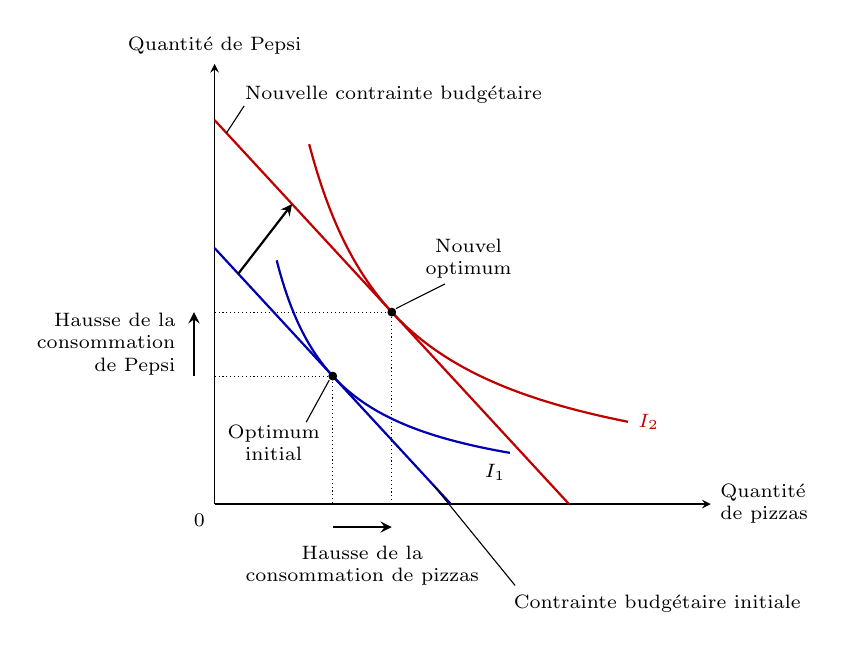
\begin{tikzpicture}[x=0.75cm,y=0.65cm,font=\scriptsize,>=stealth]
    \draw[->] (0,0) -- (8.4,0);
    \draw[->] (0,0) -- (0,8.6);
    \node[above] at (0,8.6) {Quantité de Pepsi};
    \node[right,align=left] at (8.4,0) {Quantité\\de pizzas};
    \node[below left] at (0,0) {$0$};
    % guides
    \draw[densely dotted] (0,2.5) -| (2,0);
    \draw[densely dotted] (0,3.75) -| (3,0);
    % the two contraintes budgétaires
    \draw[blue!70!black,thick] (0,5) -- (4,0);
    \draw[red!75!black,thick] (0,7.5) -- (6,0);
    \node[right] at (0.35,8.0) {Nouvelle contrainte budgétaire};
    \draw (0.5,7.78) -- (0.2,7.25);
    \node[right] (cbi) at (4.9,-1.95) {Contrainte budgétaire initiale};
    \draw ([xshift=4pt]cbi.north west) -- (3.7,0.375);
    % the two courbes d'indifférence
    \draw[blue!70!black,thick] plot[domain=1.05:5.0,samples=80] (\x,{5/\x});
    \node at (4.75,0.62) {$I_1$};
    \draw[red!75!black,thick] plot[domain=1.6:7,samples=80] (\x,{11.25/\x})
      node[right] {$I_2$};
    % the rise in income moves the contrainte budgétaire outward
    \draw[->,thick] (0.4,4.5) -- (1.31,5.86);
    % optima
    \fill (2,2.5) circle (1.6pt);
    \fill (3,3.75) circle (1.6pt);
    \node[align=center] at (1.0,1.2) {Optimum\\initial};
    \draw (1.55,1.6) -- (1.94,2.42);
    \node[align=center] at (4.3,4.8) {Nouvel\\optimum};
    \draw (3.9,4.3) -- (3.07,3.82);
    % the increase in each good
    \draw[->,thick] (2,-0.45) -- (3,-0.45);
    \node[align=center,anchor=north] at (2.5,-0.62)
      {Hausse de la\\consommation de pizzas};
    \draw[->,thick] (-0.35,2.5) -- (-0.35,3.75);
    \node[align=right,anchor=east] at (-0.5,3.125)
      {Hausse de la\\consommation\\de Pepsi};
  \end{tikzpicture}
  \caption*{\small Une hausse du revenu. The arrow between the two lines marks the
  outward move of the contrainte budgétaire, parallel to itself; the optimum passes
  from $I_1$ to $I_2$, and the arrows on the axes mark the extra pizza and the extra
  Pepsi bought.}
\end{figure}

When Pepsi becomes cheaper, the contrainte budgétaire also moves outward, but by
turning: it pivots about its end on the pizza axis, which stays put, while its end
on the Pepsi axis rises, so its slope changes. Going from the initial to the new
optimum, the consumer changes what they buy of both goods; here they buy more Pepsi
and less pizza.\\

\begin{figure}[h!]
  \centering
  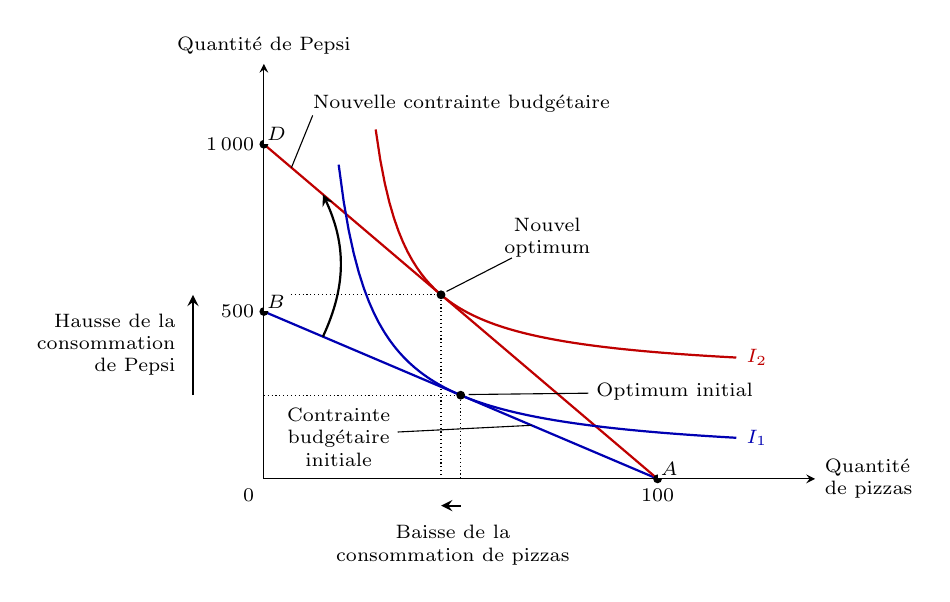
\begin{tikzpicture}[x=1.0cm,y=0.85cm,font=\scriptsize,>=stealth,
      lab/.style={fill=white,inner sep=1pt}]
    \draw[->] (0,0) -- (7,0);
    \draw[->] (0,0) -- (0,6.2);
    \node[above] at (0,6.2) {Quantité de Pepsi};
    \node[right,align=left] at (7,0) {Quantité\\de pizzas};
    \node[below left] at (0,0) {$0$};
    % guides
    \draw[densely dotted] (0,1.25) -| (2.5,0);
    \draw[densely dotted] (0,2.75) -| (2.25,0);
    % the two contraintes budgétaires
    \draw[blue!70!black,thick] (0,2.5) -- (5,0);
    \draw[red!75!black,thick] (0,5) -- (5,0);
    \node[right] at (0.5,5.6) {Nouvelle contrainte budgétaire};
    \draw (0.62,5.43) -- (0.35,4.65);
    \node[align=center] at (0.95,0.62) {Contrainte\\budgétaire\\initiale};
    \draw (1.7,0.7) -- (3.4,0.8);
    % intercepts
    \node[left] at (0,5) {$1\,000$};
    \node[left] at (0,2.5) {$500$};
    \node[below] at (5,0) {$100$};
    \fill (0,5) circle (1.6pt) node[lab,above right] {$D$};
    \fill (0,2.5) circle (1.6pt) node[lab,above right] {$B$};
    \fill (5,0) circle (1.6pt) node[lab,above right] {$A$};
    % the two courbes d'indifférence
    \draw[blue!70!black,thick] plot[domain=0.95:6,samples=80]
      (\x,{0.25+2/(\x-0.5)}) node[right] {$I_1$};
    \draw[red!75!black,thick] plot[domain=1.42:6,samples=80]
      (\x,{1.5+1.5625/(\x-1)}) node[right] {$I_2$};
    % optima
    \fill (2.5,1.25) circle (1.6pt);
    \fill (2.25,2.75) circle (1.6pt);
    \node[right] at (4.1,1.3) {Optimum initial};
    \draw (4.12,1.28) -- (2.6,1.26);
    \node[align=center] at (3.6,3.6) {Nouvel\\optimum};
    \draw (3.15,3.3) -- (2.32,2.8);
    % the fall in the price turns the contrainte budgétaire outward about A
    \draw[->,thick] (0.75,2.125) to[bend right=25] (0.75,4.25);
    % the change in each good
    \draw[->,thick] (2.5,-0.4) -- (2.25,-0.4);
    \node[align=center,anchor=north] at (2.4,-0.55)
      {Baisse de la\\consommation de pizzas};
    \draw[->,thick] (-0.9,1.25) -- (-0.9,2.75);
    \node[align=right,anchor=east] at (-1.0,2.0)
      {Hausse de la\\consommation\\de Pepsi};
  \end{tikzpicture}
  \caption*{\small Une variation du prix. A fall in the price of Pepsi turns the
  contrainte budgétaire outward about $A$, as the curved arrow shows: its Pepsi end
  rises from $B$ (500) to $D$ (1\,000), its pizza end stays at $A$ (100). From the
  initial to the new optimum the consumer buys more Pepsi and less pizza, as the
  arrows on the axes mark.}
\end{figure}

The \textbf{effets de substitution} (\textit{substitution effects}) and the
\textbf{effets de revenu} (\textit{income effects}) split the response to the
price change in two. The effet de substitution moves the consumer
along a courbe d'indifférence, to a point where the TMS is different: here from $A$
to $B$ on $I_1$. The effet de revenu carries them onto a higher courbe
d'indifférence: here from $B$, on $I_1$, to $C$, on $I_2$.

\begin{center}
\begin{minipage}{\textwidth}
  \centering
  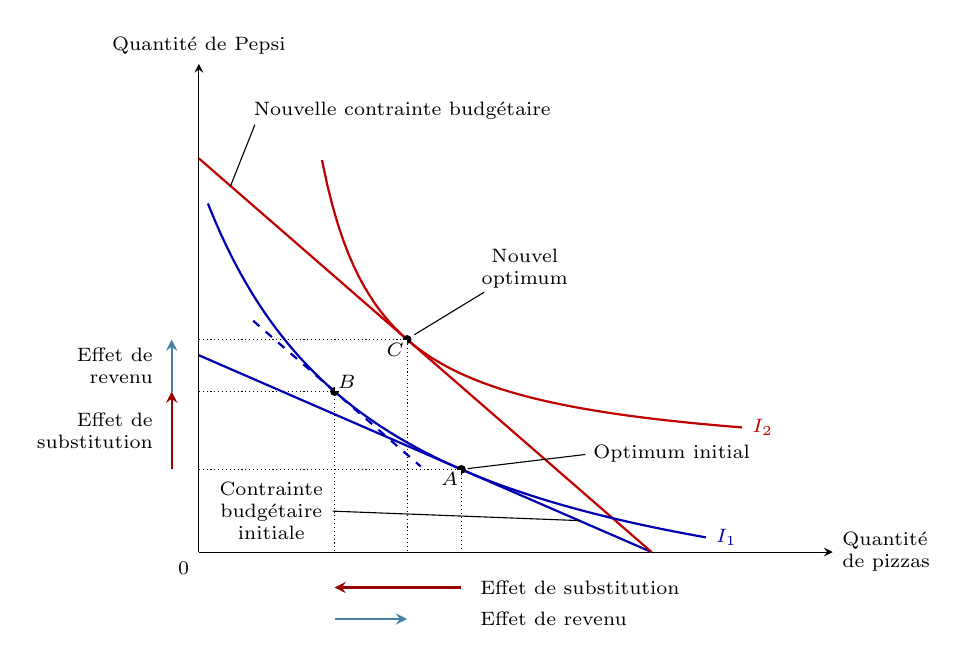
\begin{tikzpicture}[x=1.15cm,y=1.0cm,font=\scriptsize,>=stealth,
      lab/.style={fill=white,inner sep=1pt}]
    \draw[->] (0,0) -- (7,0);
    \draw[->] (0,0) -- (0,6.2);
    \node[above] at (0,6.2) {Quantité de Pepsi};
    \node[right,align=left] at (7,0) {Quantité\\de pizzas};
    \node[below left] at (0,0) {$0$};
    % guides
    \draw[densely dotted] (0,1.05) -| (2.9,0);
    \draw[densely dotted] (0,2.039) -| (1.499,0);
    \draw[densely dotted] (0,2.7) -| (2.3,0);
    % the two contraintes budgétaires and the dashed line through B
    \draw[blue!70!black,thick] (0,2.5) -- (5,0);
    \draw[red!75!black,thick] (0,5) -- (5,0);
    \draw[blue!70!black,thick,dashed] (0.6,2.938) -- (2.45,1.088);
    \node[right] at (0.5,5.6) {Nouvelle contrainte budgétaire};
    \draw (0.62,5.43) -- (0.35,4.65);
    \node[align=center] (cbi) at (0.8,0.52) {Contrainte\\budgétaire\\initiale};
    \draw (cbi.east) -- (4.2,0.4);
    % the two courbes d'indifférence
    \draw[blue!70!black,thick] plot[domain=0.1:5.6,samples=80]
      (\x,{-1.34+11.42/(\x+1.88)}) node[right] {$I_1$};
    \draw[red!75!black,thick] plot[domain=1.36:6,samples=80]
      (\x,{1.1+2.56/(\x-0.7)}) node[right] {$I_2$};
    % points
    \fill (2.9,1.05) circle (1.6pt) node[lab,below left] {$A$};
    \fill (1.499,2.039) circle (1.6pt) node[lab,above right] {$B$};
    \fill (2.3,2.7) circle (1.6pt) node[lab,below left] {$C$};
    \node[right] at (4.25,1.25) {Optimum initial};
    \draw (4.27,1.24) -- (2.97,1.06);
    \node[align=center] at (3.6,3.6) {Nouvel\\optimum};
    \draw (3.15,3.3) -- (2.38,2.76);
    % effects on the Pepsi axis
    \draw[->,thick,red!60!black] (-0.3,1.05) -- (-0.3,2.039);
    \draw[->,thick,cyan!60!black] (-0.3,2.039) -- (-0.3,2.7);
    \node[left,align=right] at (-0.4,1.545) {Effet de\\substitution};
    \node[left,align=right] at (-0.4,2.37) {Effet de\\revenu};
    % effects on the pizza axis
    \draw[->,thick,red!60!black] (2.9,-0.45) -- (1.499,-0.45);
    \draw[->,thick,cyan!60!black] (1.499,-0.85) -- (2.3,-0.85);
    \node[right] at (3.0,-0.45) {Effet de substitution};
    \node[right] at (3.0,-0.85) {Effet de revenu};
  \end{tikzpicture}
  \captionof*{figure}{\small Effets de revenu et de substitution. The effet de substitution
  moves the consumer along $I_1$ from $A$ to $B$, where the dashed line, parallel to
  the new contrainte budgétaire, touches $I_1$; the effet de revenu moves them from
  $B$ on $I_1$ to $C$ on $I_2$. On each axis, the arrows split the change of that
  good into the two effects.}
\end{minipage}
\end{center}

\subsubsection{Construction de la fonction de demande}

The optimum du consommateur yields their demand: the courbe de demande records how
the quantité demandée at the optimum goes with the price, and point by point the
optima build the \textbf{fonction de demande} (\textit{demand function}).

\begin{example}[Une baisse du prix du Pepsi]
  The price of Pepsi drops from 2~\$ to 1~\$. In panel (a), the optimum moves from
  $A$ to $B$, and the consumer buys 750 pints of Pepsi instead of 250. Panel (b)
  plots the two pairs of price and quantity, as the points $A$ and $B$ of their courbe
  de demande de Pepsi.
\end{example}

\begin{figure}[h!]
  \centering
  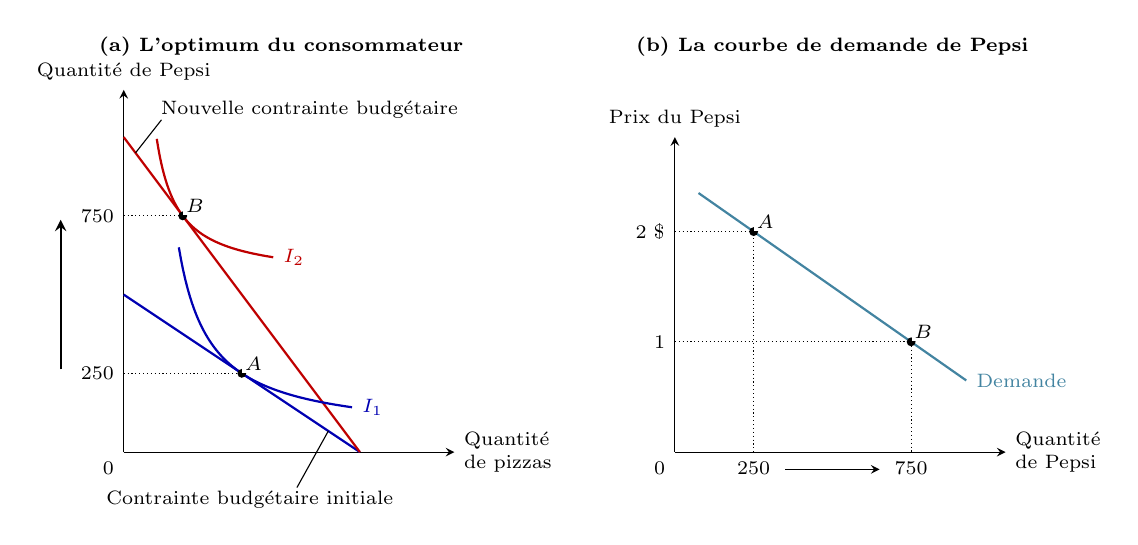
\begin{tikzpicture}[font=\scriptsize,>=stealth,
      lab/.style={fill=white,inner sep=1pt}]
    % (a) the optimum du consommateur
    \begin{scope}
      \node[font=\scriptsize\bfseries] at (2,5.15) {(a) L'optimum du consommateur};
      \draw[->] (0,0) -- (4.2,0);
      \draw[->] (0,0) -- (0,4.6);
      \node[above] at (0,4.6) {Quantité de Pepsi};
      \node[right,align=left] at (4.2,0) {Quantité\\de pizzas};
      \node[below left] at (0,0) {$0$};
      \draw[densely dotted] (0,1) -- (1.5,1);
      \draw[densely dotted] (0,3) -- (0.75,3);
      \node[left] at (0,1) {$250$};
      \node[left] at (0,3) {$750$};
      \draw[->,thick] (-0.8,1.05) -- (-0.8,2.95);
      \draw[blue!70!black,thick] (0,2) -- (3,0);
      \draw[red!75!black,thick] (0,4) -- (3,0);
      \draw[blue!70!black,thick] plot[domain=0.7:2.9,samples=80]
        (\x,{0.2+0.96/(\x-0.3)}) node[right] {$I_1$};
      \draw[red!75!black,thick] plot[domain=0.42:1.9,samples=80]
        (\x,{2.2+0.48/(\x-0.15)}) node[right] {$I_2$};
      \node[right] at (0.35,4.35) {Nouvelle contrainte budgétaire};
      \draw (0.48,4.22) -- (0.15,3.8);
      \node at (1.6,-0.6) {Contrainte budgétaire initiale};
      \draw (2.2,-0.45) -- (2.6,0.27);
      \fill (1.5,1) circle (1.6pt) node[lab,above right] {$A$};
      \fill (0.75,3) circle (1.6pt) node[lab,above right] {$B$};
    \end{scope}
    % (b) the courbe de demande
    \begin{scope}[xshift=7cm]
      \node[font=\scriptsize\bfseries] at (2,5.15) {(b) La courbe de demande de Pepsi};
      \draw[->] (0,0) -- (4.2,0);
      \draw[->] (0,0) -- (0,4.0);
      \node[above] at (0,4.0) {Prix du Pepsi};
      \node[right,align=left] at (4.2,0) {Quantité\\de Pepsi};
      \node[below left] at (0,0) {$0$};
      \draw[densely dotted] (0,2.8) -| (1,0);
      \draw[densely dotted] (0,1.4) -| (3,0);
      \node[left] at (0,2.8) {$2$~\$};
      \node[left] at (0,1.4) {$1$};
      \node[below] at (1,0) {$250$};
      \node[below] at (3,0) {$750$};
      \draw[->] (1.4,-0.22) -- (2.6,-0.22);
      \draw[cyan!60!black,thick] (0.3,3.29) -- (3.7,0.91) node[right] {Demande};
      \fill (1,2.8) circle (1.6pt) node[lab,above right] {$A$};
      \fill (3,1.4) circle (1.6pt) node[lab,above right] {$B$};
    \end{scope}
  \end{tikzpicture}
  \caption*{\small Construction de la courbe de demande. Each optimum of panel (a)
  gives one point of panel (b): at 2~\$ the consumer buys 250 pints of Pepsi ($A$),
  at 1~\$ they buy 750 ($B$).}
\end{figure}

\subsection{La demande agrégée}

At each price, the quantité demandée in a market adds up what every buyer demands
at that price. The courbe de la \textbf{demande agrégée} (\textit{market demand}) is
therefore the horizontal sum of the individual courbes de demande.

\begin{example}[La demande de cornets de Catherine et de Nicholas]
  At each price, the quantité demandée in the market is the sum of Catherine's and
  Nicholas's; Catherine's column is the barème de demande above.
  \begin{center}
    \begin{tabular}{@{}cccccc@{}}
      \toprule
      Prix du cornet de glace & Catherine & & Nicholas & & Marché \\
      \midrule
      $0{,}00$~\$ & 12 & $+$ & 7 & $=$ & 19 cornets \\
      $0{,}50$ & 10 & & 6 & & 16 \\
      $1{,}00$ & 8 & & 5 & & 13 \\
      $1{,}50$ & 6 & & 4 & & 10 \\
      $2{,}00$ & 4 & & 3 & & 7 \\
      $2{,}50$ & 2 & & 2 & & 4 \\
      $3{,}00$ & 0 & & 1 & & 1 \\
      \bottomrule
    \end{tabular}
  \end{center}
  At 2,00~\$, Catherine buys 4 cones and Nicholas 3: the market demands 7 cones at
  that price.
\end{example}

\begin{figure}[h!]
  \centering
  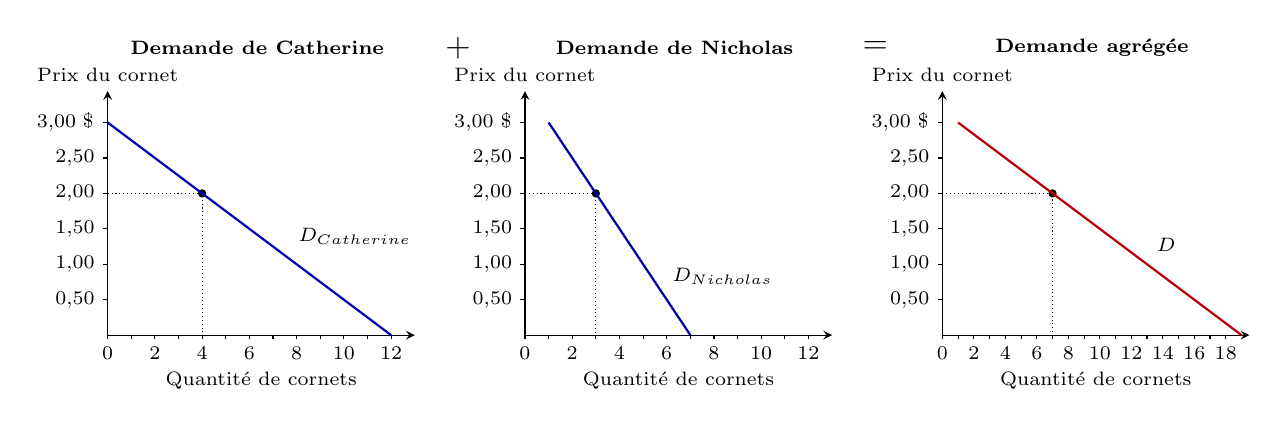
\begin{tikzpicture}[font=\scriptsize,>=stealth]
    \foreach \s/\ttl/\m/\n/\pt/\lab/\lx/\ly in {
        0/{Demande de Catherine}/0.3/12/4/{$D_{\text{Catherine}}$}/2.3/1.25,
        5.3/{Demande de Nicholas}/0.3/12/3/{$D_{\text{Nicholas}}$}/1.75/0.75,
        10.6/{Demande agrégée}/0.2/18/7/{$D$}/2.6/1.15} {
      \begin{scope}[xshift=\s cm]
        \node[font=\scriptsize\bfseries] at (1.9,3.65) {\ttl};
        \draw[->] (0,0) -- (3.9,0);
        \draw[->] (0,0) -- (0,3.1);
        \node[above] at (0,3.1) {Prix du cornet};
        \node[below] at (1.95,-0.35) {Quantité de cornets};
        \foreach \p/\l in {0.45/{0,50},0.9/{1,00},1.35/{1,50},1.8/{2,00},
            2.25/{2,50},2.7/{3,00~\$}}
          { \draw (0,\p) -- (-0.06,\p); \node[left] at (-0.04,\p) {\l}; }
        \foreach \q in {0,...,\n} \draw ({\m*\q},0) -- ({\m*\q},-0.05);
        \foreach \q in {0,2,...,\n} \node[below] at ({\m*\q},-0.03) {\q};
        \draw[densely dotted] (0,1.8) -| ({\m*\pt},0);
        \fill ({\m*\pt},1.8) circle (1.5pt);
        \node[right] at (\lx,\ly) {\lab};
      \end{scope}
    }
    % the three curves
    \draw[blue!70!black,thick] (0,2.7) -- (3.6,0);
    \draw[blue!70!black,thick] (5.6,2.7) -- (7.4,0);
    \draw[red!75!black,thick] (10.8,2.7) -- (14.4,0);
    \node[font=\large] at (4.45,3.65) {$+$};
    \node[font=\large] at (9.75,3.65) {$=$};
  \end{tikzpicture}
  \caption*{\small La demande agrégée, somme horizontale des demandes
  individuelles. At each price the quantities demanded by Catherine and Nicholas
  add up to the market's: at 2,00~\$, $4 + 3 = 7$ cones.}
\end{figure}

\subsection{Déplacement de la demande}

A \textbf{déplacement de la demande} (\textit{shift in demand}) moves the whole
courbe de demande. Whatever makes buyers want more of the good at every price moves
the courbe de demande to the right, from $D_1$ to $D_2$, an increase in demand;
whatever makes them want less at every price moves it to the left, from $D_1$ to
$D_3$, a decrease in demand.

\begin{figure}[h!]
  \centering
  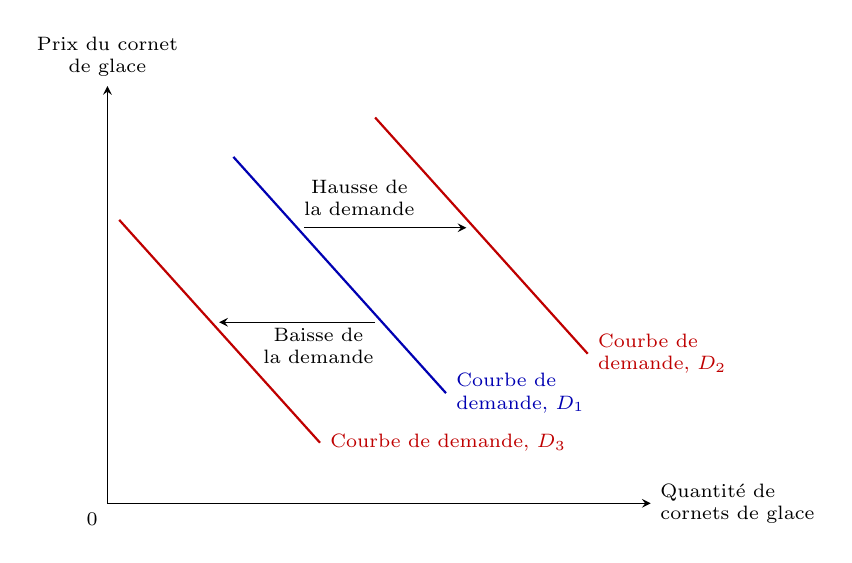
\begin{tikzpicture}[font=\scriptsize,>=stealth]
    \draw[->] (0,0) -- (6.9,0);
    \draw[->] (0,0) -- (0,5.3);
    \node[above,align=center] at (0,5.3) {Prix du cornet\\de glace};
    \node[right,align=left] at (6.9,0) {Quantité de\\cornets de glace};
    \node[below left] at (0,0) {$0$};
    \draw[red!75!black,thick] (0.15,3.6) -- (2.7,0.77)
      node[right] {Courbe de demande, $D_3$};
    \draw[blue!70!black,thick] (1.6,4.4) -- (4.3,1.4)
      node[right,align=left] {Courbe de\\demande, $D_1$};
    \draw[red!75!black,thick] (3.4,4.9) -- (6.1,1.9)
      node[right,align=left] {Courbe de\\demande, $D_2$};
    \draw[->] (2.5,3.5) -- (4.56,3.5);
    \node[align=center] at (3.2,3.88) {Hausse de\\la demande};
    \draw[->] (3.4,2.3) -- (1.42,2.3);
    \node[align=center] at (2.68,2.0) {Baisse de\\la demande};
  \end{tikzpicture}
  \caption*{\small Déplacements de la courbe de demande. An increase in demand
  shifts the curve to the right, from $D_1$ to $D_2$; a decrease shifts it to the
  left, from $D_1$ to $D_3$.}
\end{figure}

\subsection{Élasticité de la demande}

\begin{definition}[Élasticité de la demande (\textit{price elasticity of demand})]
  \leavevmode
  \begin{itemize}
    \item Effet en pourcentage~: si le prix augmente de 1~\%, de combien diminue la
      demande en~\%.
    \item Donne la sensibilité au prix.
  \end{itemize}
  \[ -\,\frac{\text{variation en \% de la quantité demandée}}{\text{variation en \%
     du prix}} \]
  \[ -\,\frac{\Delta Q}{Q} \bigg/ \frac{\Delta P}{P} = -\,\frac{P}{Q}\,
     \frac{\Delta Q}{\Delta P} \]
  \[ \varepsilon = -\,\frac{P}{Q}\,\frac{dQ}{dP} \]
\end{definition}

The definition is given in words, then with the variations $\Delta Q$ and
$\Delta P$ of the quantité demandée $Q$ and the price $P$, and last with the
derivative $\dfrac{dQ}{dP}$, which defines $\varepsilon$.\\

How steep or flat the courbe de demande is depends on the élasticité de la
demande. Five cases are distinguished. Cases (a) to (d) are drawn with the same rise
in the price, from 4~\$ to 5~\$, that is 22~\%; in case (e) the courbe de demande
is horizontal at 4~\$:
\begin{enumerate}[(a)]
  \item a demande \textbf{parfaitement inélastique} (\textit{perfectly inelastic}),
    $\varepsilon = 0$: the courbe de demande is vertical, and the rise in the price
    leaves the quantité demandée unchanged, at 100;
  \item a demande \textbf{inélastique} (\textit{inelastic}), $\varepsilon < 1$: the
    rise in the price leads to an 11~\% decrease in the quantité demandée, from 100
    to 90;
  \item a demande of \textbf{élasticité unitaire} (\textit{unit elasticity}),
    $\varepsilon = 1$: a 22~\% decrease, from 100 to 80;
  \item a demande \textbf{élastique} (\textit{elastic}), $\varepsilon > 1$: a 67~\%
    decrease, from 100 to 50;
  \item a demande \textbf{parfaitement élastique} (\textit{perfectly elastic}),
    $\varepsilon$ infinite: at any price above 4~\$ the quantité demandée is zero,
    at exactly 4~\$ consumers will buy any quantity, and at a price below 4~\$ the
    quantité demandée is infinite.
\end{enumerate}
All these percentages are computed by the \textbf{méthode du point milieu}
(\textit{midpoint method}), which divides each change by the average of the
starting and the final value.

\begin{figure}[h!]
  \centering
  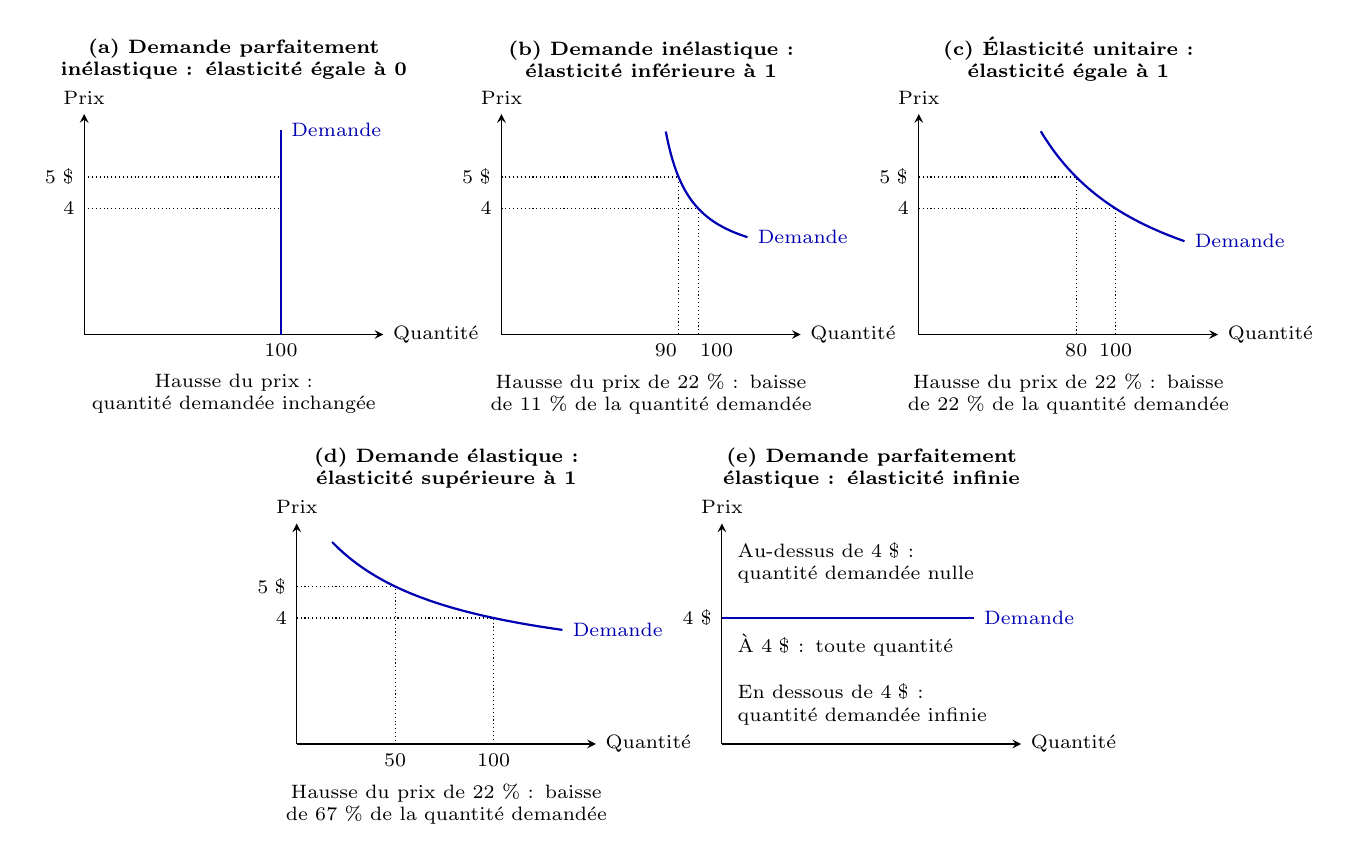
\begin{tikzpicture}[font=\scriptsize,>=stealth,
      ttl/.style={text width=5cm,align=center,font=\scriptsize\bfseries},
      ann/.style={text width=4.8cm,align=center,anchor=north}]
    % (a) parfaitement inélastique
    \begin{scope}
      \node[ttl] at (1.9,3.5) {(a) Demande parfaitement\\inélastique~: élasticité égale à 0};
      \draw[->] (0,0) -- (3.8,0);
      \draw[->] (0,0) -- (0,2.8);
      \node[above] at (0,2.8) {Prix};
      \node[right] at (3.8,0) {Quantité};
      \draw[densely dotted] (0,1.6) -- (2.5,1.6);
      \draw[densely dotted] (0,2.0) -- (2.5,2.0);
      \node[left] at (0,1.6) {4};
      \node[left] at (0,2.0) {5~\$};
      \draw[blue!70!black,thick] (2.5,0) -- (2.5,2.6) node[right] {Demande};
      \node[below] at (2.5,0) {100};
      \node[ann] at (1.9,-0.38) {Hausse du prix~:\\quantité demandée inchangée};
    \end{scope}
    % (b) inélastique
    \begin{scope}[xshift=5.3cm]
      \node[ttl] at (1.9,3.5) {(b) Demande inélastique~:\\élasticité inférieure à 1};
      \draw[->] (0,0) -- (3.8,0);
      \draw[->] (0,0) -- (0,2.8);
      \node[above] at (0,2.8) {Prix};
      \node[right] at (3.8,0) {Quantité};
      \draw[densely dotted] (0,2.0) -| (2.25,0);
      \draw[densely dotted] (0,1.6) -| (2.5,0);
      \node[left] at (0,1.6) {4};
      \node[left] at (0,2.0) {5~\$};
      \draw[blue!70!black,thick] plot[domain=83.5:125,samples=60]
        ({0.025*\x},{0.4*(2+60/(\x-70))}) node[right] {Demande};
      \node[below left,inner xsep=1pt] at (2.27,0) {90};
      \node[below right,inner xsep=1pt] at (2.48,0) {100};
      \node[ann] at (1.9,-0.38) {Hausse du prix de 22~\%~: baisse\\de 11~\% de la quantité demandée};
    \end{scope}
    % (c) élasticité unitaire
    \begin{scope}[xshift=10.6cm]
      \node[ttl] at (1.9,3.5) {(c) Élasticité unitaire~:\\élasticité égale à 1};
      \draw[->] (0,0) -- (3.8,0);
      \draw[->] (0,0) -- (0,2.8);
      \node[above] at (0,2.8) {Prix};
      \node[right] at (3.8,0) {Quantité};
      \draw[densely dotted] (0,2.0) -| (2.0,0);
      \draw[densely dotted] (0,1.6) -| (2.5,0);
      \node[left] at (0,1.6) {4};
      \node[left] at (0,2.0) {5~\$};
      \draw[blue!70!black,thick] plot[domain=62:135,samples=60]
        ({0.025*\x},{0.4*400/\x}) node[right] {Demande};
      \node[below] at (2.0,0) {80};
      \node[below] at (2.5,0) {100};
      \node[ann] at (1.9,-0.38) {Hausse du prix de 22~\%~: baisse\\de 22~\% de la quantité demandée};
    \end{scope}
    % (d) élastique
    \begin{scope}[xshift=2.7cm,yshift=-5.2cm]
      \node[ttl] at (1.9,3.5) {(d) Demande élastique~:\\élasticité supérieure à 1};
      \draw[->] (0,0) -- (3.8,0);
      \draw[->] (0,0) -- (0,2.8);
      \node[above] at (0,2.8) {Prix};
      \node[right] at (3.8,0) {Quantité};
      \draw[densely dotted] (0,2.0) -| (1.25,0);
      \draw[densely dotted] (0,1.6) -| (2.5,0);
      \node[left] at (0,1.6) {4};
      \node[left] at (0,2.0) {5~\$};
      \draw[blue!70!black,thick] plot[domain=18:135,samples=60]
        ({0.025*\x},{0.4*(2+300/(\x+50))}) node[right] {Demande};
      \node[below] at (1.25,0) {50};
      \node[below] at (2.5,0) {100};
      \node[ann] at (1.9,-0.38) {Hausse du prix de 22~\%~: baisse\\de 67~\% de la quantité demandée};
    \end{scope}
    % (e) parfaitement élastique
    \begin{scope}[xshift=8.1cm,yshift=-5.2cm]
      \node[ttl] at (1.9,3.5) {(e) Demande parfaitement\\élastique~: élasticité infinie};
      \draw[->] (0,0) -- (3.8,0);
      \draw[->] (0,0) -- (0,2.8);
      \node[above] at (0,2.8) {Prix};
      \node[right] at (3.8,0) {Quantité};
      \node[left] at (0,1.6) {4~\$};
      \draw[blue!70!black,thick] (0,1.6) -- (3.2,1.6) node[right] {Demande};
      \node[text width=3.3cm,align=left] at (1.85,2.3) {Au-dessus de 4~\$~:\\quantité demandée nulle};
      \node[text width=3.3cm,align=left] at (1.85,1.25) {À 4~\$~: toute quantité};
      \node[text width=3.3cm,align=left] at (1.85,0.5) {En dessous de 4~\$~:\\quantité demandée infinie};
    \end{scope}
  \end{tikzpicture}
  \caption*{\small L'élasticité de la demande, de 0 à l'infini. From (a) to (d),
  the same rise in the price, from 4~\$ to 5~\$, meets an ever flatter courbe de
  demande and brings an ever larger fall in the quantité demandée; in (e) the courbe
  de demande is horizontal at 4~\$.}
\end{figure}

\subsection{L'offre}

Supply is set out as demand was, starting from one seller, Ben, whose
\textbf{barème d'offre} (\textit{supply schedule}) lists, price by price, the
\textbf{quantité offerte} (\textit{quantity supplied}). The \textbf{courbe d'offre}
(\textit{supply curve}) draws the barème d'offre as a graph, the quantité offerte of
the good against its price. It slopes upward: the dearer the good, the larger the
quantité offerte.

\begin{example}[Le barème d'offre de Ben]
  Ben's barème d'offre for ice-cream cones:
  \begin{center}
    \begin{tabular}{@{}cc@{}}
      \toprule
      Prix du cornet de glace & Quantité de cornets offerte \\
      \midrule
      $0{,}00$~\$ & 0 cornet \\
      $0{,}50$ & 0 \\
      $1{,}00$ & 1 \\
      $1{,}50$ & 2 \\
      $2{,}00$ & 3 \\
      $2{,}50$ & 4 \\
      $3{,}00$ & 5 \\
      \bottomrule
    \end{tabular}
  \end{center}
  A rise in the price from 2,00 to 2,50~\$ raises Ben's quantité offerte from 3 to 4
  cones.
\end{example}

\begin{figure}[h!]
  \centering
  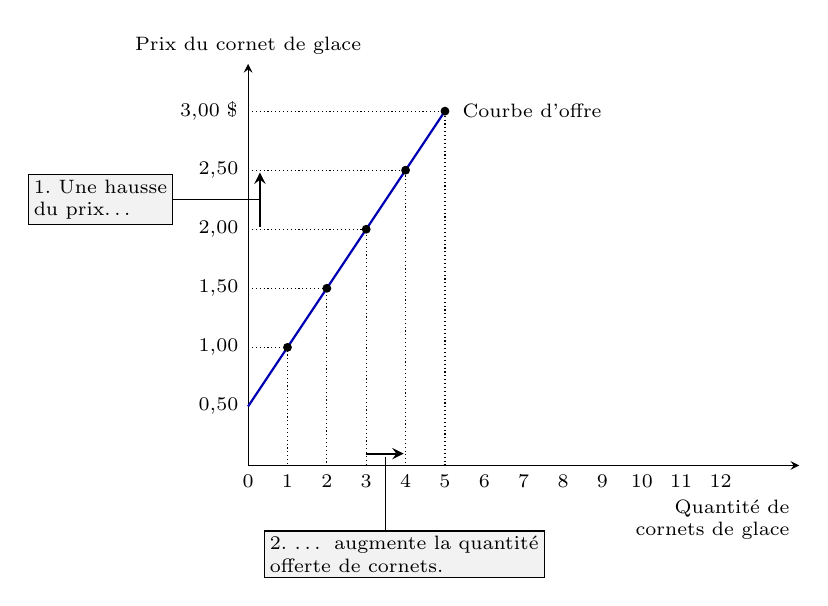
\begin{tikzpicture}[x=0.5cm,y=1.5cm,font=\scriptsize,>=stealth,
      call/.style={draw,fill=black!5,align=left,inner sep=2pt}]
    \draw[->] (0,0) -- (14,0);
    \draw[->] (0,0) -- (0,3.4);
    \node[above] at (0,3.4) {Prix du cornet de glace};
    \node[below left,align=right] at (14,-0.21) {Quantité de\\cornets de glace};
    \foreach \q in {0,...,12} \node[below] at (\q,0) {$\q$};
    \foreach \p/\l in {0.5/{$0{,}50$},1/{$1{,}00$},1.5/{$1{,}50$},2/{$2{,}00$},
        2.5/{$2{,}50$},3/{$3{,}00$~\$}}
      \node[left] at (0,\p) {\l};
    \foreach \k in {1,...,5} \draw[densely dotted] (0,{0.5+0.5*\k}) -| (\k,0);
    \draw[blue!70!black,thick] (0,0.5) -- (5,3);
    \foreach \k in {1,...,5} \fill (\k,{0.5+0.5*\k}) circle (1.6pt);
    \node[right] at (5.2,3) {Courbe d'offre};
    % a rise in the price raises the quantity supplied
    \draw[->,thick] (0.3,2.02) -- (0.3,2.48);
    \node[call,anchor=east] (c1) at (-1.9,2.25) {1.\ Une hausse\\du prix\ldots};
    \draw (c1.east) -- (0.3,2.25);
    \draw[->,thick] (3,0.1) -- (3.95,0.1);
    \node[call,anchor=north west] (c2) at (0.4,-0.55)
      {2.\ \ldots{} augmente la quantité\\offerte de cornets.};
    \draw (3.5,-0.55) -- (3.5,0.07);
  \end{tikzpicture}
  \caption*{\small L'offre individuelle de Ben. The barème d'offre plotted point by
  point; a higher price raises the quantité offerte, so the courbe d'offre slopes
  upward.}
\end{figure}

\subsubsection{Élasticité de l'offre}

\begin{figure}[h!]
  \centering
  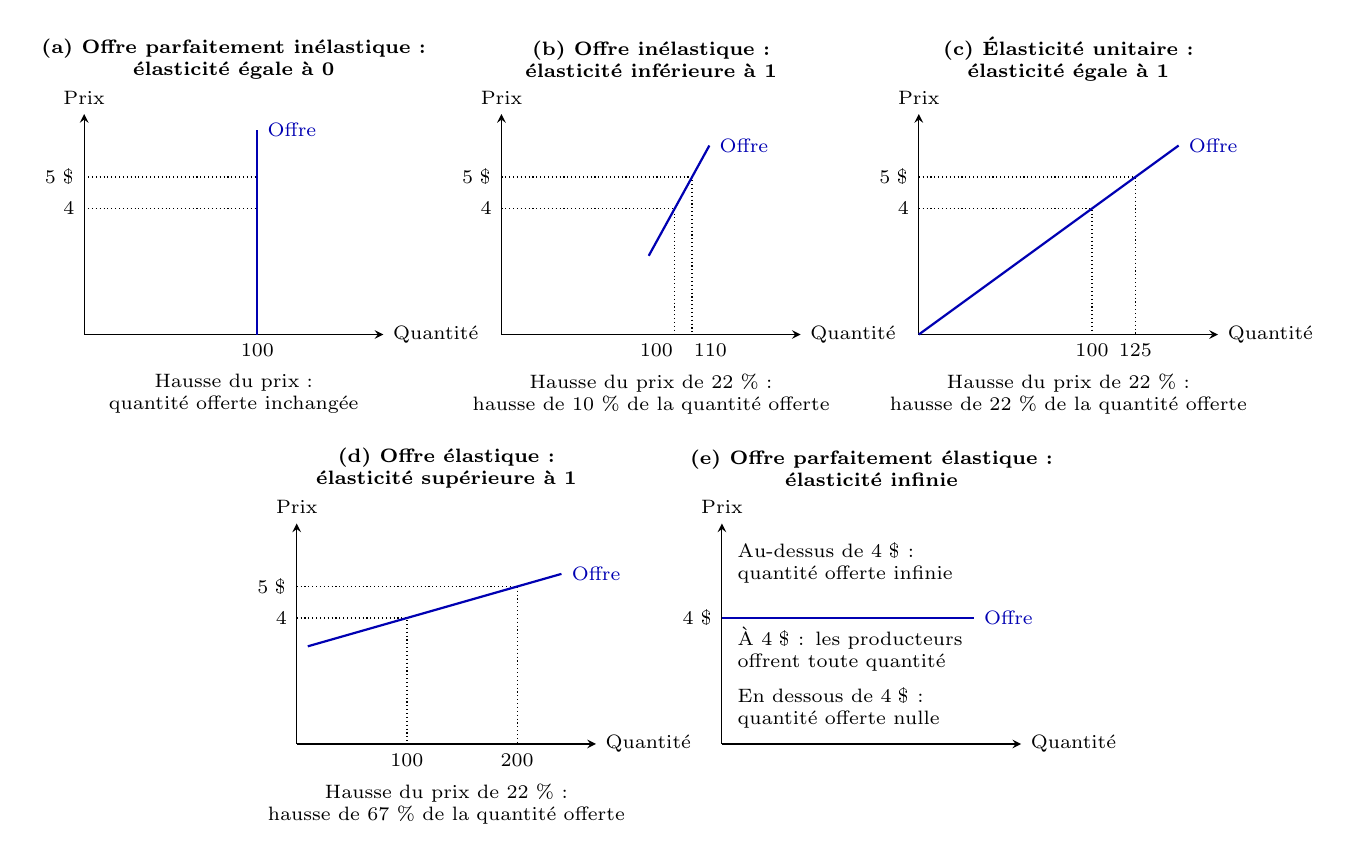
\begin{tikzpicture}[font=\scriptsize,>=stealth,
      ttl/.style={text width=5cm,align=center,font=\scriptsize\bfseries},
      ann/.style={text width=4.8cm,align=center,anchor=north}]
    % (a) parfaitement inélastique
    \begin{scope}
      \node[ttl] at (1.9,3.5) {(a) Offre parfaitement inélastique~:\\élasticité égale à 0};
      \draw[->] (0,0) -- (3.8,0);
      \draw[->] (0,0) -- (0,2.8);
      \node[above] at (0,2.8) {Prix};
      \node[right] at (3.8,0) {Quantité};
      \draw[densely dotted] (0,1.6) -- (2.2,1.6);
      \draw[densely dotted] (0,2.0) -- (2.2,2.0);
      \node[left] at (0,1.6) {4};
      \node[left] at (0,2.0) {5~\$};
      \draw[blue!70!black,thick] (2.2,0) -- (2.2,2.6) node[right] {Offre};
      \node[below] at (2.2,0) {100};
      \node[ann] at (1.9,-0.38) {Hausse du prix~:\\quantité offerte inchangée};
    \end{scope}
    % (b) inélastique
    \begin{scope}[xshift=5.3cm]
      \node[ttl] at (1.9,3.5) {(b) Offre inélastique~:\\élasticité inférieure à 1};
      \draw[->] (0,0) -- (3.8,0);
      \draw[->] (0,0) -- (0,2.8);
      \node[above] at (0,2.8) {Prix};
      \node[right] at (3.8,0) {Quantité};
      \draw[densely dotted] (0,1.6) -| (2.2,0);
      \draw[densely dotted] (0,2.0) -| (2.42,0);
      \node[left] at (0,1.6) {4};
      \node[left] at (0,2.0) {5~\$};
      \draw[blue!70!black,thick] plot[domain=85:120,samples=2]
        ({0.022*\x},{0.4*(4+(\x-100)/10)}) node[right] {Offre};
      \node[below left,inner xsep=1pt] at (2.22,0) {100};
      \node[below right,inner xsep=1pt] at (2.4,0) {110};
      \node[ann] at (1.9,-0.38) {Hausse du prix de 22~\%~:\\hausse de 10~\% de la quantité offerte};
    \end{scope}
    % (c) élasticité unitaire
    \begin{scope}[xshift=10.6cm]
      \node[ttl] at (1.9,3.5) {(c) Élasticité unitaire~:\\élasticité égale à 1};
      \draw[->] (0,0) -- (3.8,0);
      \draw[->] (0,0) -- (0,2.8);
      \node[above] at (0,2.8) {Prix};
      \node[right] at (3.8,0) {Quantité};
      \draw[densely dotted] (0,1.6) -| (2.2,0);
      \draw[densely dotted] (0,2.0) -| (2.75,0);
      \node[left] at (0,1.6) {4};
      \node[left] at (0,2.0) {5~\$};
      \draw[blue!70!black,thick] (0,0) -- (3.3,2.4) node[right] {Offre};
      \node[below] at (2.2,0) {100};
      \node[below] at (2.75,0) {125};
      \node[ann] at (1.9,-0.38) {Hausse du prix de 22~\%~:\\hausse de 22~\% de la quantité offerte};
    \end{scope}
    % (d) élastique
    \begin{scope}[xshift=2.7cm,yshift=-5.2cm]
      \node[ttl] at (1.9,3.5) {(d) Offre élastique~:\\élasticité supérieure à 1};
      \draw[->] (0,0) -- (3.8,0);
      \draw[->] (0,0) -- (0,2.8);
      \node[above] at (0,2.8) {Prix};
      \node[right] at (3.8,0) {Quantité};
      \draw[densely dotted] (0,1.6) -| (1.4,0);
      \draw[densely dotted] (0,2.0) -| (2.8,0);
      \node[left] at (0,1.6) {4};
      \node[left] at (0,2.0) {5~\$};
      \draw[blue!70!black,thick] plot[domain=10:240,samples=2]
        ({0.014*\x},{0.4*(3+\x/100)}) node[right] {Offre};
      \node[below] at (1.4,0) {100};
      \node[below] at (2.8,0) {200};
      \node[ann] at (1.9,-0.38) {Hausse du prix de 22~\%~:\\hausse de 67~\% de la quantité offerte};
    \end{scope}
    % (e) parfaitement élastique
    \begin{scope}[xshift=8.1cm,yshift=-5.2cm]
      \node[ttl] at (1.9,3.5) {(e) Offre parfaitement élastique~:\\élasticité infinie};
      \draw[->] (0,0) -- (3.8,0);
      \draw[->] (0,0) -- (0,2.8);
      \node[above] at (0,2.8) {Prix};
      \node[right] at (3.8,0) {Quantité};
      \node[left] at (0,1.6) {4~\$};
      \draw[blue!70!black,thick] (0,1.6) -- (3.2,1.6) node[right] {Offre};
      \node[text width=3.3cm,align=left] at (1.85,2.3) {Au-dessus de 4~\$~:\\quantité offerte infinie};
      \node[text width=3.3cm,align=left] at (1.85,1.2) {À 4~\$~: les producteurs\\offrent toute quantité};
      \node[text width=3.3cm,align=left] at (1.85,0.45) {En dessous de 4~\$~:\\quantité offerte nulle};
    \end{scope}
  \end{tikzpicture}
  \caption*{\small L'élasticité de l'offre, de 0 à l'infini. From (a) to (d), the
  same rise in the price, from 4~\$ to 5~\$, meets an ever flatter courbe d'offre
  and brings an ever larger rise in the quantité offerte; in (e) the courbe d'offre
  is horizontal at 4~\$.}
\end{figure}

How steep or flat the courbe d'offre is depends on the \textbf{élasticité de
l'offre} (\textit{price elasticity of supply}). The same five cases are drawn, with
percentages computed by the méthode du point milieu: in cases (a) to (d), again a
rise in the price from 4~\$ to 5~\$, that is 22~\%; in case (e), a horizontal
courbe d'offre at 4~\$:
\begin{enumerate}[(a)]
  \item an offre parfaitement inélastique, élasticité égale à 0: the courbe d'offre
    is vertical, and the rise in the price leaves the quantité offerte unchanged, at
    100;
  \item an offre inélastique, élasticité inférieure à 1: the rise in the price leads
    to a 10~\% increase in the quantité offerte, from 100 to 110;
  \item élasticité unitaire, égale à 1: the courbe d'offre is a straight line
    through the origin, and the quantité offerte rises by 22~\%, from 100 to 125;
  \item an offre élastique, élasticité supérieure à 1: a 67~\% increase, from 100
    to 200;
  \item an offre parfaitement élastique, élasticité infinie: at any price above
    4~\$ the quantité offerte is infinite, at exactly 4~\$ producers will supply any
    quantity, and at a price below 4~\$ the quantité offerte is zero.
\end{enumerate}

\subsubsection{Facteurs influençant l'offre}

Four factors influence supply; they are named, not developed:
\begin{itemize}
  \item le prix des inputs et les coûts~;
  \item la technologie~;
  \item les anticipations~;
  \item le nombre de vendeurs et la concurrence.
\end{itemize}
The first is at work in the example of the price of sugar, with the déplacement de
l'équilibre.

\subsubsection{Déplacement de l'offre}

A \textbf{déplacement de l'offre} (\textit{shift in supply}) moves the whole courbe
d'offre. Whatever makes sellers want to produce more at every price moves the
courbe d'offre to the right, from $S_1$ to $S_2$, an increase in supply; whatever
makes them want to produce less at every price moves it to the left, from $S_1$ to
$S_3$, a decrease in supply.

\begin{figure}[h!]
  \centering
  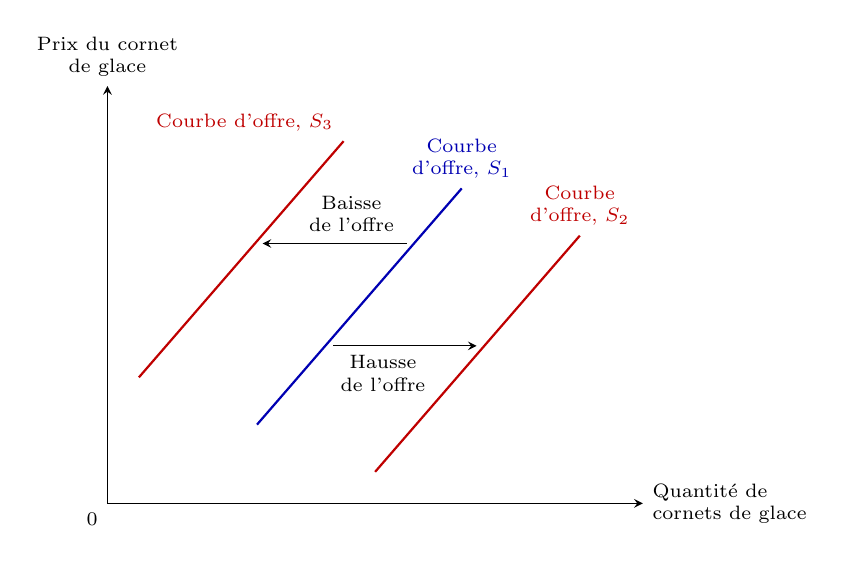
\begin{tikzpicture}[font=\scriptsize,>=stealth]
    \draw[->] (0,0) -- (6.8,0);
    \draw[->] (0,0) -- (0,5.3);
    \node[above,align=center] at (0,5.3) {Prix du cornet\\de glace};
    \node[right,align=left] at (6.8,0) {Quantité de\\cornets de glace};
    \node[below left] at (0,0) {$0$};
    \draw[red!75!black,thick] (0.4,1.6) -- (3.0,4.6)
      node[above left] {Courbe d'offre, $S_3$};
    \draw[blue!70!black,thick] (1.9,1.0) -- (4.5,4.0)
      node[above,align=center] {Courbe\\d'offre, $S_1$};
    \draw[red!75!black,thick] (3.4,0.4) -- (6.0,3.4)
      node[above,align=center] {Courbe\\d'offre, $S_2$};
    \draw[->] (3.8,3.3) -- (1.97,3.3);
    \node[align=center] at (3.1,3.68) {Baisse\\de l'offre};
    \draw[->] (2.87,2.0) -- (4.69,2.0);
    \node[align=center] at (3.5,1.65) {Hausse\\de l'offre};
  \end{tikzpicture}
  \caption*{\small Déplacements de la courbe d'offre. An increase in supply shifts
  the curve to the right, from $S_1$ to $S_2$; a decrease shifts it to the left,
  from $S_1$ to $S_3$.}
\end{figure}

\subsection{L'équilibre de marché}

The courbe d'offre and the courbe de demande cross at the \textbf{équilibre de
marché} (\textit{market equilibrium}), also called the équilibre concurrentiel. At
the price where they cross, the \textbf{prix d'équilibre} (\textit{equilibrium
price}), buyers want exactly what sellers offer: the quantité offerte and the
quantité demandée are equal, and their common value is the \textbf{quantité
d'équilibre} (\textit{equilibrium quantity}). In the market for ice-cream cones of
the figure, the prix d'équilibre is 2,00~\$, and at that price sellers offer 7
cones and buyers want 7.\\

\begin{figure}[h!]
  \centering
  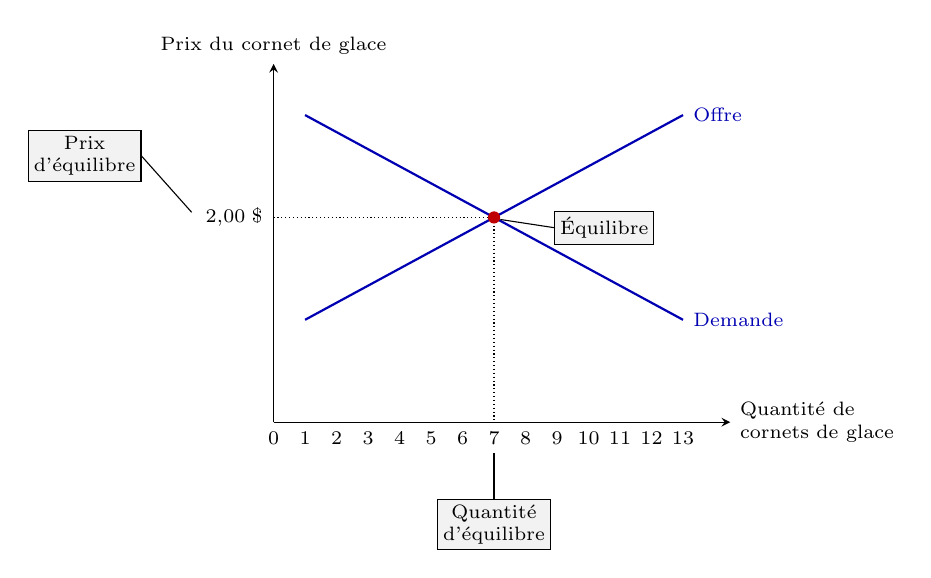
\begin{tikzpicture}[x=0.4cm,y=1.3cm,font=\scriptsize,>=stealth,
      call/.style={draw,fill=black!5,align=center,inner sep=2pt}]
    \draw[->] (0,0) -- (14.5,0);
    \draw[->] (0,0) -- (0,3.5);
    \node[above] at (0,3.5) {Prix du cornet de glace};
    \node[right,align=left] at (14.5,0) {Quantité de\\cornets de glace};
    \foreach \q in {0,...,13} \node[below] at (\q,0) {$\q$};
    \draw[densely dotted] (0,2) -| (7,0);
    \node[left] at (0,2) {$2{,}00$~\$};
    \draw[blue!70!black,thick] (1,3) -- (13,1) node[right] {Demande};
    \draw[blue!70!black,thick] (1,1) -- (13,3) node[right] {Offre};
    \fill[red!75!black] (7,2) circle (2.2pt);
    \node[call] (e) at (10.5,1.9) {Équilibre};
    \draw (e.west) -- (7.2,1.98);
    \node[call] (p) at (-6,2.6) {Prix\\d'équilibre};
    \draw (p.east) -- (-2.6,2.05);
    \node[call] (q) at (7,-1.0) {Quantité\\d'équilibre};
    \draw (q.north) -- (7,-0.3);
  \end{tikzpicture}
  \caption*{\small L'équilibre de l'offre et de la demande. The two curves cross at
  the prix d'équilibre, 2,00~\$, and the quantité d'équilibre, 7 cones.}
\end{figure}

At any other price the market is out of equilibrium, and the price moves. Above the
prix d'équilibre, the quantité offerte exceeds the quantité demandée, and the gap is
an \textbf{excédent} (\textit{surplus}); sellers then cut the price to sell more,
which brings it down towards the prix d'équilibre. Below the prix d'équilibre, the
quantité demandée exceeds the quantité offerte, and the gap is a \textbf{pénurie}
(\textit{shortage}); with buyers competing for too few goods, sellers can raise the
price. Either way, the movement of the price pushes the market back to the
équilibre de marché.

\begin{figure}[h!]
  \centering
  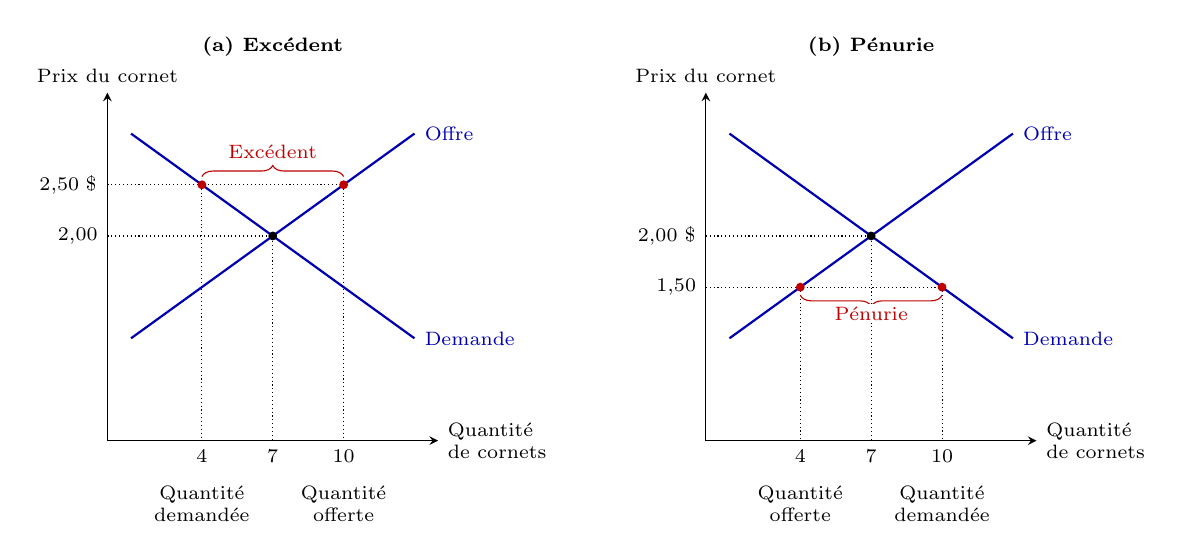
\begin{tikzpicture}[x=0.3cm,y=1.3cm,font=\scriptsize,>=stealth,
      brc/.style={decorate,decoration={brace,amplitude=4pt}}]
    % (a) excédent
    \begin{scope}
      \node[font=\scriptsize\bfseries] at (7,3.85) {(a) Excédent};
      \draw[->] (0,0) -- (14,0);
      \draw[->] (0,0) -- (0,3.4);
      \node[above] at (0,3.4) {Prix du cornet};
      \node[right,align=left] at (14,0) {Quantité\\de cornets};
      \draw[blue!70!black,thick] (1,3) -- (13,1) node[right] {Demande};
      \draw[blue!70!black,thick] (1,1) -- (13,3) node[right] {Offre};
      \draw[densely dotted] (0,2) -| (7,0);
      \draw[densely dotted] (0,2.5) -- (10,2.5);
      \draw[densely dotted] (4,2.5) -- (4,0);
      \draw[densely dotted] (10,2.5) -- (10,0);
      \fill (7,2) circle (1.6pt);
      \fill[red!75!black] (4,2.5) circle (1.6pt);
      \fill[red!75!black] (10,2.5) circle (1.6pt);
      \draw[brc,red!75!black] (4,2.58) -- (10,2.58)
        node[midway,above=3pt] {Excédent};
      \node[left] at (0,2) {$2{,}00$};
      \node[left] at (0,2.5) {$2{,}50$~\$};
      \foreach \q in {4,7,10} \node[below] at (\q,0) {$\q$};
      \node[align=center] at (4,-0.62) {Quantité\\demandée};
      \node[align=center] at (10,-0.62) {Quantité\\offerte};
    \end{scope}
    % (b) pénurie
    \begin{scope}[xshift=7.6cm]
      \node[font=\scriptsize\bfseries] at (7,3.85) {(b) Pénurie};
      \draw[->] (0,0) -- (14,0);
      \draw[->] (0,0) -- (0,3.4);
      \node[above] at (0,3.4) {Prix du cornet};
      \node[right,align=left] at (14,0) {Quantité\\de cornets};
      \draw[blue!70!black,thick] (1,3) -- (13,1) node[right] {Demande};
      \draw[blue!70!black,thick] (1,1) -- (13,3) node[right] {Offre};
      \draw[densely dotted] (0,2) -| (7,0);
      \draw[densely dotted] (0,1.5) -- (10,1.5);
      \draw[densely dotted] (4,1.5) -- (4,0);
      \draw[densely dotted] (10,1.5) -- (10,0);
      \fill (7,2) circle (1.6pt);
      \fill[red!75!black] (4,1.5) circle (1.6pt);
      \fill[red!75!black] (10,1.5) circle (1.6pt);
      \draw[brc,red!75!black] (10,1.42) -- (4,1.42)
        node[midway,below=3pt,fill=white,inner sep=1pt] {Pénurie};
      \node[left] at (0,2) {$2{,}00$~\$};
      \node[left] at (0,1.5) {$1{,}50$};
      \foreach \q in {4,7,10} \node[below] at (\q,0) {$\q$};
      \node[align=center] at (4,-0.62) {Quantité\\offerte};
      \node[align=center] at (10,-0.62) {Quantité\\demandée};
    \end{scope}
  \end{tikzpicture}
  \caption*{\small Des marchés hors de l'équilibre. Above the prix d'équilibre the
  quantité offerte exceeds the quantité demandée, an excédent (a); below it the
  quantité demandée exceeds the quantité offerte, a pénurie (b).}
\end{figure}

\begin{example}[Un marché des cornets hors de l'équilibre]
  At 2,50~\$, above the prix d'équilibre, 10 cones are supplied and 4 demanded: an
  excédent. At 1,50~\$, below it, 10 cones are demanded and 4 supplied: a pénurie.
\end{example}

\subsubsection{Déplacement de l'équilibre}

A déplacement de la demande or de l'offre moves the équilibre de marché. If some
event makes buyers want more at every price, the courbe de demande moves right, and
the prix d'équilibre and the quantité d'équilibre both go up.

\begin{example}[Un été caniculaire]
  An unusually hot summer makes buyers want more ice cream. The courbe de demande
  moves from $D_1$ to $D_2$: the prix d'équilibre goes up from 2,00 to 2,50~\$ and
  the quantité d'équilibre from 7 to 10 cones.
\end{example}

\begin{figure}[h!]
  \centering
  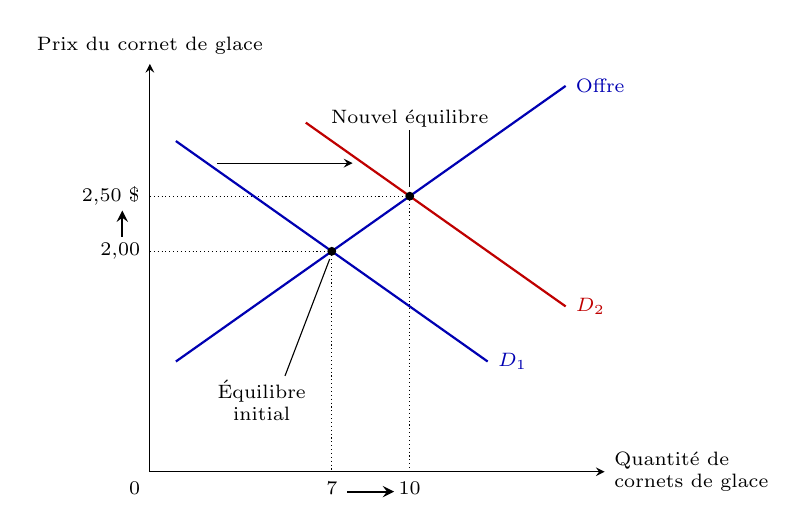
\begin{tikzpicture}[x=0.33cm,y=1.4cm,font=\scriptsize,>=stealth]
    \draw[->] (0,0) -- (17.5,0);
    \draw[->] (0,0) -- (0,3.7);
    \node[above] at (0,3.7) {Prix du cornet de glace};
    \node[right,align=left] at (17.5,0) {Quantité de\\cornets de glace};
    \node[below left] at (0,0) {$0$};
    \draw[densely dotted] (0,2) -| (7,0);
    \draw[densely dotted] (0,2.5) -| (10,0);
    \node[left] at (0,2) {$2{,}00$};
    \node[left] at (0,2.5) {$2{,}50$~\$};
    \node[below] at (7,0) {$7$};
    \node[below] at (10,0) {$10$};
    \draw[blue!70!black,thick] (1,1) -- (16,3.5) node[right] {Offre};
    \draw[blue!70!black,thick] (1,3) -- (13,1) node[right] {$D_1$};
    \draw[red!75!black,thick] (6,3.167) -- (16,1.5) node[right] {$D_2$};
    \draw[->] (2.6,2.8) -- (7.8,2.8);
    \fill (7,2) circle (1.6pt);
    \fill (10,2.5) circle (1.6pt);
    \node[align=center] at (4.3,0.65) {Équilibre\\initial};
    \draw (5.2,0.87) -- (6.92,1.93);
    \node at (10,3.2) {Nouvel équilibre};
    \draw (10,3.1) -- (10,2.58);
    % the rise in the price and in the quantity
    \draw[->,thick] (-1.06,2.13) -- (-1.06,2.37);
    \draw[->,thick] (7.6,-0.18) -- (9.4,-0.18);
  \end{tikzpicture}
  \caption*{\small Une hausse de la demande. Hot weather moves the courbe de demande
  from $D_1$ to $D_2$ along an unchanged courbe d'offre; the arrows on the axes mark
  the rise in the price and in the quantity sold.}
\end{figure}

If instead some event makes sellers offer less at every price, the courbe d'offre
moves left: the prix d'équilibre goes up and the quantité d'équilibre goes down.

\begin{figure}[h!]
  \centering
  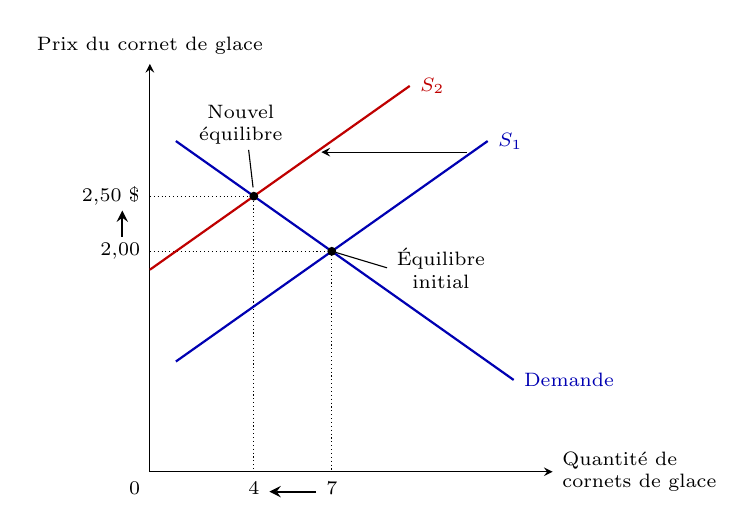
\begin{tikzpicture}[x=0.33cm,y=1.4cm,font=\scriptsize,>=stealth]
    \draw[->] (0,0) -- (15.5,0);
    \draw[->] (0,0) -- (0,3.7);
    \node[above] at (0,3.7) {Prix du cornet de glace};
    \node[right,align=left] at (15.5,0) {Quantité de\\cornets de glace};
    \node[below left] at (0,0) {$0$};
    \draw[densely dotted] (0,2) -| (7,0);
    \draw[densely dotted] (0,2.5) -| (4,0);
    \node[left] at (0,2) {$2{,}00$};
    \node[left] at (0,2.5) {$2{,}50$~\$};
    \node[below] at (4,0) {$4$};
    \node[below] at (7,0) {$7$};
    \draw[blue!70!black,thick] (1,3) -- (14,0.833) node[right] {Demande};
    \draw[blue!70!black,thick] (1,1) -- (13,3) node[right] {$S_1$};
    \draw[red!75!black,thick] (0,1.833) -- (10,3.5) node[right] {$S_2$};
    \draw[->] (12.2,2.9) -- (6.6,2.9);
    \fill (7,2) circle (1.6pt);
    \fill (4,2.5) circle (1.6pt);
    \node[align=center] (ei) at (11.2,1.85) {Équilibre\\initial};
    \draw (ei.west) -- (7.15,1.99);
    \node[align=center] at (3.5,3.15) {Nouvel\\équilibre};
    \draw (3.8,2.92) -- (3.97,2.58);
    % the rise in the price and the fall in the quantity
    \draw[->,thick] (-1.06,2.13) -- (-1.06,2.37);
    \draw[->,thick] (6.4,-0.18) -- (4.6,-0.18);
  \end{tikzpicture}
  \caption*{\small Une baisse de l'offre. Dearer sugar moves the courbe d'offre from
  $S_1$ to $S_2$ along an unchanged courbe de demande; the arrows on the axes mark
  the rise in the price and the fall in the quantity sold.}
\end{figure}

\begin{example}[Une hausse du prix du sucre]
  Sugar is an input of ice cream; when its price goes up, sellers offer less ice
  cream, the first of the facteurs influençant l'offre at work. The courbe d'offre
  moves from $S_1$ to $S_2$: the prix d'équilibre goes up from 2,00 to 2,50~\$ and
  the quantité d'équilibre down from 7 to 4 cones.
\end{example}

\begin{figure}[h!]
  \centering
  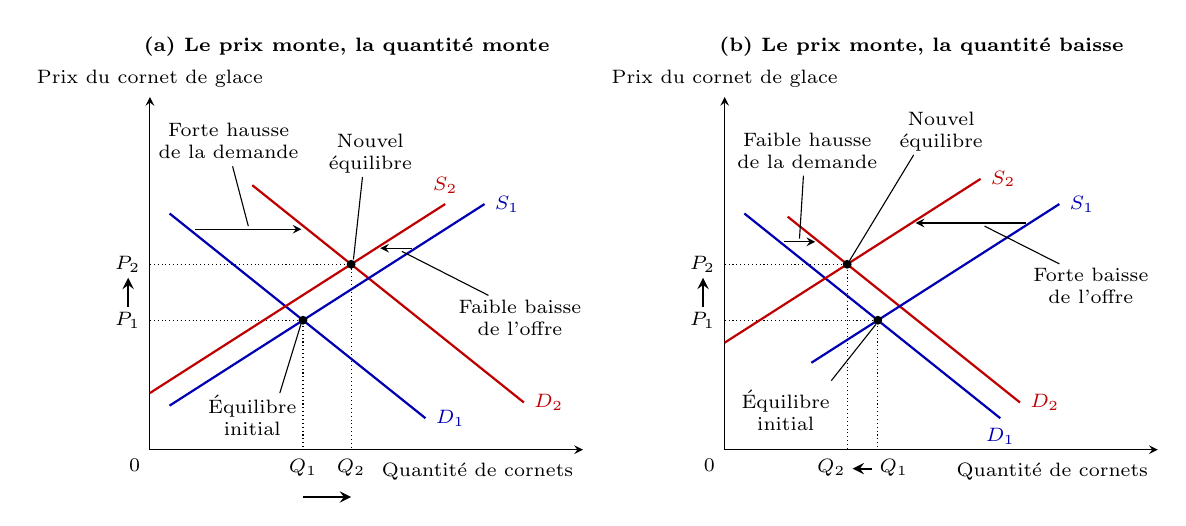
\begin{tikzpicture}[x=0.5cm,y=0.8cm,font=\scriptsize,>=stealth]
    % (a) le prix monte, la quantité monte
    \begin{scope}
      \node[font=\scriptsize\bfseries] at (5,6.4) {(a) Le prix monte, la quantité monte};
      \draw[->] (0,0) -- (11,0);
      \draw[->] (0,0) -- (0,5.6);
      \node[above] at (0,5.6) {Prix du cornet de glace};
      \node[below left] at (11,-0.05) {Quantité de cornets};
      \node[below left] at (0,0) {$0$};
      \draw[densely dotted] (0,2.056) -| (3.889,0);
      \draw[densely dotted] (0,2.944) -| (5.111,0);
      \node[left] at (0,2.056) {$P_1$};
      \node[left] at (0,2.944) {$P_2$};
      \node[below] at (3.889,0) {$Q_1$};
      \node[below] at (5.111,0) {$Q_2$};
      \draw[blue!70!black,thick] (0.5,3.75) -- (7,0.5) node[right] {$D_1$};
      \draw[red!75!black,thick] (2.6,4.2) -- (9.5,0.75) node[right] {$D_2$};
      \draw[blue!70!black,thick] (0.5,0.7) -- (8.5,3.9) node[right] {$S_1$};
      \draw[red!75!black,thick] (0,0.9) -- (7.5,3.9) node[above] {$S_2$};
      \fill (3.889,2.056) circle (1.6pt);
      \fill (5.111,2.944) circle (1.6pt);
      \draw[->] (1.15,3.5) -- (3.85,3.5);
      \node[align=center] at (2.0,4.9) {Forte hausse\\de la demande};
      \draw (2.1,4.5) -- (2.5,3.55);
      \draw[->] (6.65,3.2) -- (5.85,3.2);
      \node[align=center] at (9.4,2.1) {Faible baisse\\de l'offre};
      \draw (8.6,2.45) -- (6.4,3.15);
      % the two equilibria
      \node[align=center] at (2.6,0.55) {Équilibre\\initial};
      \draw (3.3,0.9) -- (3.84,2.0);
      \node[align=center] at (5.6,4.7) {Nouvel\\équilibre};
      \draw (5.4,4.33) -- (5.17,3.02);
      % the rise in the price and in the quantity
      \draw[->,thick] (-0.55,2.27) -- (-0.55,2.73);
      \draw[->,thick] (3.889,-0.75) -- (5.111,-0.75);
    \end{scope}
    % (b) le prix monte, la quantité baisse
    \begin{scope}[xshift=7.3cm]
      \node[font=\scriptsize\bfseries] at (5,6.4) {(b) Le prix monte, la quantité baisse};
      \draw[->] (0,0) -- (11,0);
      \draw[->] (0,0) -- (0,5.6);
      \node[above] at (0,5.6) {Prix du cornet de glace};
      \node[below left] at (11,-0.05) {Quantité de cornets};
      \node[below left] at (0,0) {$0$};
      \draw[densely dotted] (0,2.056) -| (3.889,0);
      \draw[densely dotted] (0,2.944) -| (3.111,0);
      \node[left] at (0,2.056) {$P_1$};
      \node[left] at (0,2.944) {$P_2$};
      \node[below right,inner xsep=1pt] at (3.85,0) {$Q_1$};
      \node[below left,inner xsep=1pt] at (3.15,0) {$Q_2$};
      \draw[blue!70!black,thick] (0.5,3.75) -- (7,0.5) node[below] {$D_1$};
      \draw[red!75!black,thick] (1.6,3.7) -- (7.5,0.75) node[right] {$D_2$};
      \draw[blue!70!black,thick] (2.2,1.38) -- (8.5,3.9) node[right] {$S_1$};
      \draw[red!75!black,thick] (0,1.7) -- (6.5,4.3) node[right] {$S_2$};
      \fill (3.889,2.056) circle (1.6pt);
      \fill (3.111,2.944) circle (1.6pt);
      \draw[->] (1.5,3.3) -- (2.3,3.3);
      \node[align=center] at (2.1,4.75) {Faible hausse\\de la demande};
      \draw (2.0,4.35) -- (1.9,3.35);
      \draw[->] (7.65,3.6) -- (4.85,3.6);
      \node[align=center] at (9.3,2.6) {Forte baisse\\de l'offre};
      \draw (8.5,2.95) -- (6.6,3.55);
      % the two equilibria
      \node[align=center] (eib) at (1.55,0.62) {Équilibre\\initial};
      \draw ([xshift=-3pt]eib.north east) -- (3.84,1.99);
      \node[align=center] at (5.5,5.05) {Nouvel\\équilibre};
      \draw (4.8,4.68) -- (3.17,3.0);
      % the rise in the price and the fall in the quantity
      \draw[->,thick] (-0.55,2.27) -- (-0.55,2.73);
      \draw[->,thick] (3.75,-0.3) -- (3.25,-0.3);
    \end{scope}
  \end{tikzpicture}
  \caption*{\small Un déplacement de l'offre et de la demande. In both panels demand
  rises and supply falls, and the price goes up from $P_1$ to $P_2$; the quantity
  goes up in (a) and down in (b), depending on which déplacement is the larger.}
\end{figure}

If demand rises and supply falls at once, either of two outcomes can follow. With a
large rise in demand and a small fall in supply, panel (a), the prix d'équilibre
goes up from $P_1$ to $P_2$ and so does the quantité d'équilibre, from $Q_1$ to
$Q_2$. With a small rise in demand and a large fall in supply, panel (b), the prix
d'équilibre still goes up from $P_1$ to $P_2$, but the quantité d'équilibre goes
down from $Q_1$ to $Q_2$.

\subsection{Contrôle des prix}

Two kinds of intervention follow: the contrôle des prix, which brings rationnement,
here, and taxes, in the next subsection. Their figures for the market for ice-cream
cones share another équilibre de marché, at 3~\$ and 100 cones, distinct from the
2,00~\$ and 7 cones above.\\

Under a \textbf{contrôle des prix} (\textit{price controls}), the government sets a
limit on the market price: a \textbf{prix plafond} (\textit{price ceiling}), above
which the price may not rise, or a \textbf{prix plancher} (\textit{price floor}),
below which it may not fall.

\subsubsection{Prix plafonds}

Set above the prix d'équilibre, a prix plafond changes nothing: it is not
\textbf{contraignant} (\textit{binding}), and the market settles at its équilibre de
marché. Set below the prix d'équilibre, it is contraignant: the market price is
held at the prix plafond, the quantité demandée exceeds the quantité offerte, and
there is a pénurie.

\begin{example}[Un prix plafond sur le marché des cornets]
  With a prix plafond of 4~\$, panel (a), the prix plafond sits above the prix
  d'équilibre of 3~\$ and changes nothing: 100 cones are offered and 100 demanded.
  With a prix plafond of 2~\$, panel (b), the prix plafond sits below the prix
  d'équilibre, and the market price is held at 2~\$. Buyers then want 125 cones but
  sellers offer only 75: a pénurie of 50 cones.
\end{example}

\begin{figure}[h!]
  \centering
  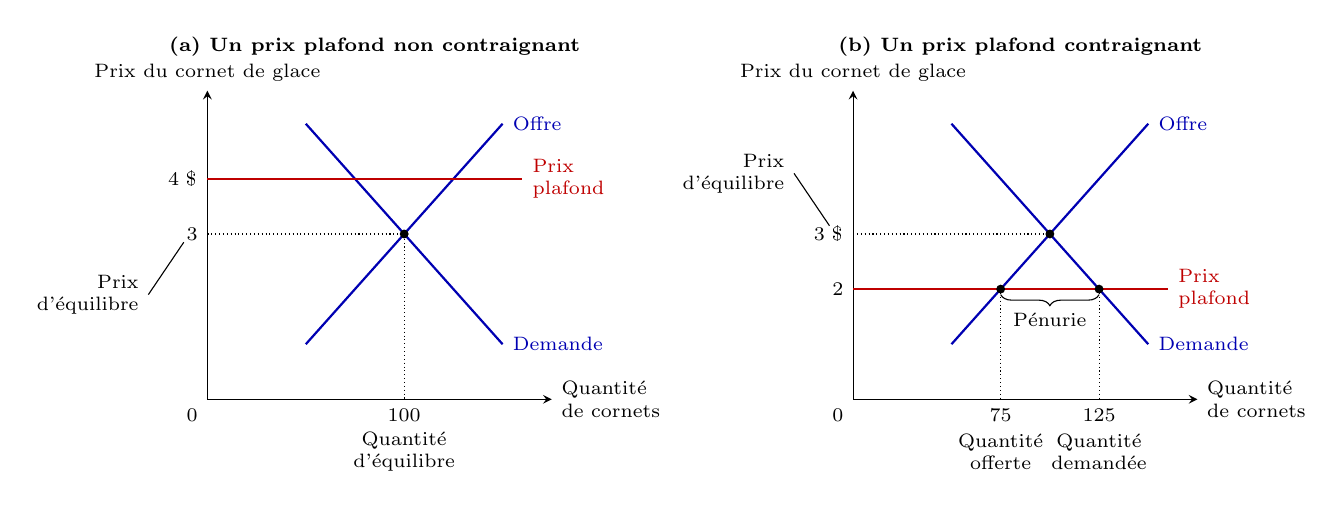
\begin{tikzpicture}[x=0.025cm,y=0.7cm,font=\scriptsize,>=stealth,
      brc/.style={decorate,decoration={brace,amplitude=4pt}}]
    % (a) non contraignant
    \begin{scope}
      \node[font=\scriptsize\bfseries] at (85,6.4) {(a) Un prix plafond non contraignant};
      \draw[->] (0,0) -- (175,0);
      \draw[->] (0,0) -- (0,5.6);
      \node[above] at (0,5.6) {Prix du cornet de glace};
      \node[right,align=left] at (175,0) {Quantité\\de cornets};
      \node[below left] at (0,0) {$0$};
      \draw[blue!70!black,thick] (50,1) -- (150,5) node[right] {Offre};
      \draw[blue!70!black,thick] (50,5) -- (150,1) node[right] {Demande};
      \draw[red!75!black,thick] (0,4) -- (160,4) node[right,align=left] {Prix\\plafond};
      \draw[densely dotted] (0,3) -| (100,0);
      \fill (100,3) circle (1.6pt);
      \node[left] at (0,3) {$3$};
      \node[left] at (0,4) {$4$~\$};
      \node[below] at (100,0) {$100$};
      \node[align=right,anchor=east] (pe) at (-30,1.9) {Prix\\d'équilibre};
      \draw (pe.east) -- (-12,2.85);
      \node[align=center] at (100,-0.95) {Quantité\\d'équilibre};
    \end{scope}
    % (b) contraignant
    \begin{scope}[xshift=8.2cm]
      \node[font=\scriptsize\bfseries] at (85,6.4) {(b) Un prix plafond contraignant};
      \draw[->] (0,0) -- (175,0);
      \draw[->] (0,0) -- (0,5.6);
      \node[above] at (0,5.6) {Prix du cornet de glace};
      \node[right,align=left] at (175,0) {Quantité\\de cornets};
      \node[below left] at (0,0) {$0$};
      \draw[blue!70!black,thick] (50,1) -- (150,5) node[right] {Offre};
      \draw[blue!70!black,thick] (50,5) -- (150,1) node[right] {Demande};
      \draw[red!75!black,thick] (0,2) -- (160,2) node[right,align=left] {Prix\\plafond};
      \draw[densely dotted] (0,3) -- (100,3);
      \draw[densely dotted] (75,2) -- (75,0);
      \draw[densely dotted] (125,2) -- (125,0);
      \fill (100,3) circle (1.6pt);
      \fill (75,2) circle (1.6pt);
      \fill (125,2) circle (1.6pt);
      \draw[brc] (125,1.9) -- (75,1.9) node[midway,below=3pt] {Pénurie};
      \node[left] at (0,2) {$2$};
      \node[left] at (0,3) {$3$~\$};
      \node[align=right,anchor=east] (pe) at (-30,4.1) {Prix\\d'équilibre};
      \draw (pe.east) -- (-12,3.15);
      \node[below] at (75,0) {$75$};
      \node[below] at (125,0) {$125$};
      \node[align=center] at (75,-0.95) {Quantité\\offerte};
      \node[align=center] at (125,-0.95) {Quantité\\demandée};
    \end{scope}
  \end{tikzpicture}
  \caption*{\small Un marché avec un prix plafond. Set above the prix d'équilibre
  (a), the prix plafond leaves the market at its équilibre de marché; set below it
  (b), it
  leaves a pénurie of 50 cones.}
\end{figure}

How large the pénurie is depends on the élasticité de l'offre and the élasticité de
la demande. The
\textbf{contrôle des loyers} (\textit{rent control}) is a prix plafond imposed on
the rent of apartments by a law. À court terme, the courbes d'offre and de demande
for apartments are relatively inélastiques, and the contrôle des loyers causes only
a small pénurie of housing. À long terme, they are more élastiques, and the
contrôle des loyers causes a large pénurie.

\begin{figure}[h!]
  \centering
  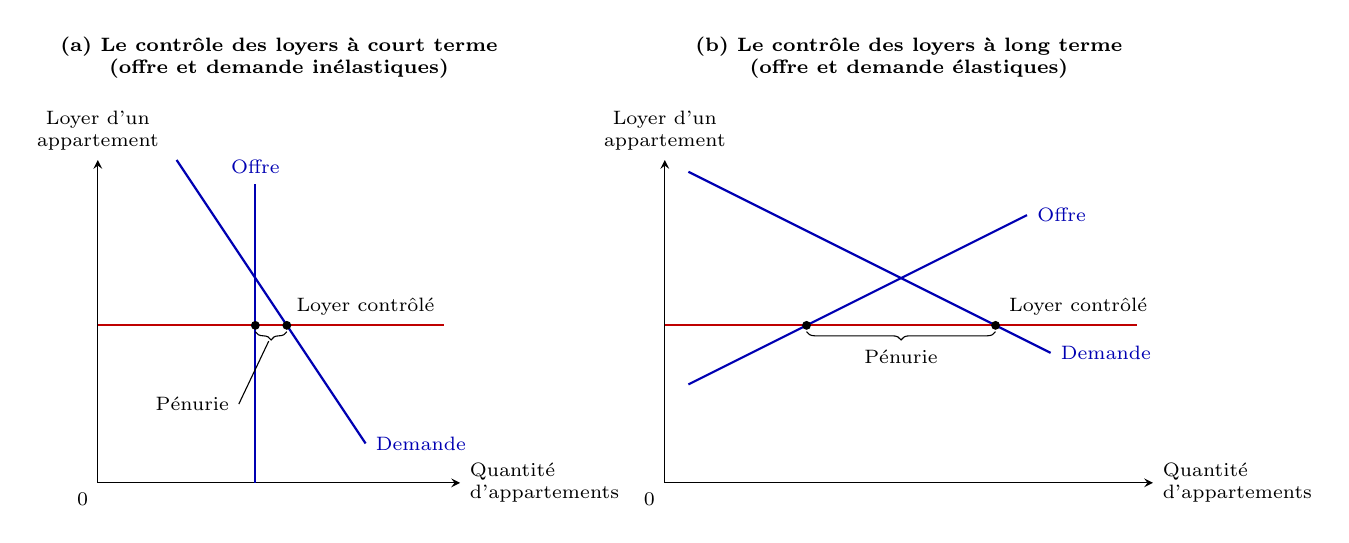
\begin{tikzpicture}[font=\scriptsize,>=stealth,
      brc/.style={decorate,decoration={brace,amplitude=3pt}},
      ttl/.style={text width=6cm,align=center,font=\scriptsize\bfseries}]
    % (a) court terme
    \begin{scope}
      \node[ttl] at (2.3,5.4) {(a) Le contrôle des loyers à court terme\\(offre et demande inélastiques)};
      \draw[->] (0,0) -- (4.6,0);
      \draw[->] (0,0) -- (0,4.1);
      \node[above,align=center] at (0,4.1) {Loyer d'un\\appartement};
      \node[right,align=left] at (4.6,0) {Quantité\\d'appartements};
      \node[below left] at (0,0) {$0$};
      \draw[blue!70!black,thick] (2,0) -- (2,3.8) node[above] {Offre};
      \draw[blue!70!black,thick] (1.0,4.1) -- (3.4,0.5) node[right] {Demande};
      \draw[red!75!black,thick] (0,2) -- (4.4,2);
      \node[above left] at (4.4,2) {Loyer contrôlé};
      \fill (2,2) circle (1.6pt);
      \fill (2.4,2) circle (1.6pt);
      \draw[brc] (2.4,1.92) -- (2,1.92);
      \node (pa) at (1.2,1.0) {Pénurie};
      \draw (pa.east) -- (2.17,1.8);
    \end{scope}
    % (b) long terme
    \begin{scope}[xshift=7.2cm]
      \node[ttl] at (3.1,5.4) {(b) Le contrôle des loyers à long terme\\(offre et demande élastiques)};
      \draw[->] (0,0) -- (6.2,0);
      \draw[->] (0,0) -- (0,4.1);
      \node[above,align=center] at (0,4.1) {Loyer d'un\\appartement};
      \node[right,align=left] at (6.2,0) {Quantité\\d'appartements};
      \node[below left] at (0,0) {$0$};
      \draw[blue!70!black,thick] (0.3,1.25) -- (4.6,3.4) node[right] {Offre};
      \draw[blue!70!black,thick] (0.3,3.95) -- (4.9,1.65) node[right] {Demande};
      \draw[red!75!black,thick] (0,2) -- (6.0,2);
      \node[above right] at (4.25,2.0) {Loyer contrôlé};
      \fill (1.8,2) circle (1.6pt);
      \fill (4.2,2) circle (1.6pt);
      \draw[brc] (4.2,1.92) -- (1.8,1.92) node[midway,below=3pt] {Pénurie};
    \end{scope}
  \end{tikzpicture}
  \caption*{\small Le contrôle des loyers à court terme et à long terme. The same
  loyer contrôlé, below the equilibrium rent, leaves a small pénurie when the courbes
  d'offre and de demande are inélastiques (a) and a large one when they are
  élastiques (b).}
\end{figure}

\subsubsection{Prix planchers}

The prix plancher is the mirror case. Set below the prix d'équilibre, it changes
nothing, and the price still settles where supply meets demand. Set above it, it is
contraignant: the market price is held at the prix plancher, the quantité offerte
exceeds the quantité demandée, and there is an excédent.

\begin{example}[Un prix plancher sur le marché des cornets]
  With a prix plancher of 2~\$, panel (a), the prix plancher sits below the prix
  d'équilibre of 3~\$ and changes nothing: at the équilibre de marché, 100 cones are
  offered and 100 demanded. With a prix plancher of 4~\$, panel (b), the prix
  plancher sits
  above the prix d'équilibre, and the market price is held at 4~\$. Sellers then
  offer 120 cones but buyers want only 80: an excédent of 40 cones.
\end{example}

\begin{figure}[h!]
  \centering
  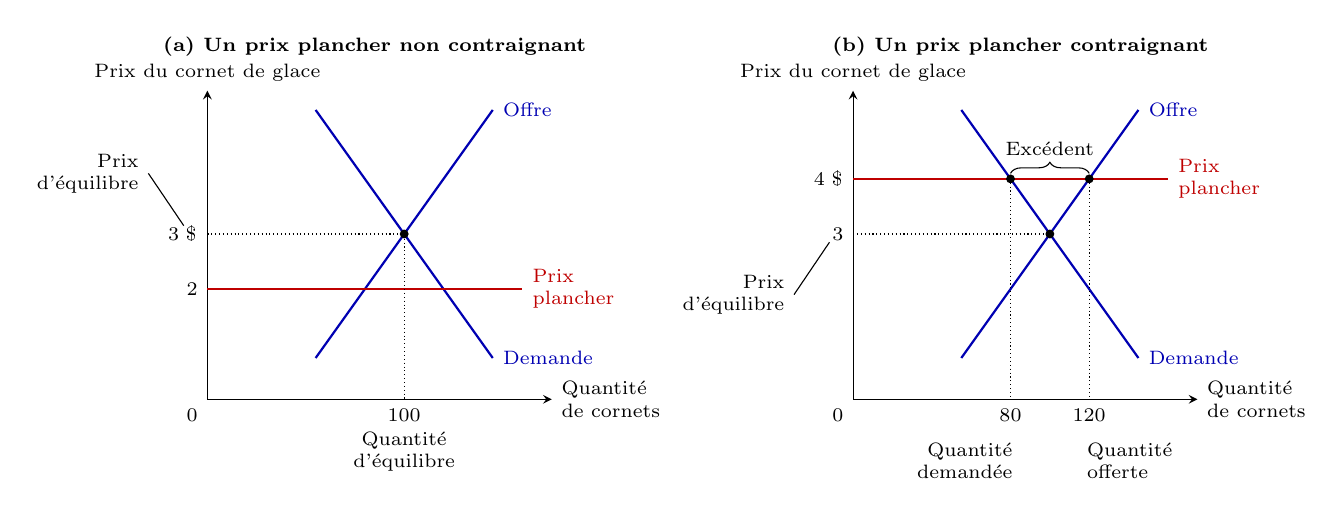
\begin{tikzpicture}[x=0.025cm,y=0.7cm,font=\scriptsize,>=stealth,
      brc/.style={decorate,decoration={brace,amplitude=4pt}}]
    % (a) non contraignant
    \begin{scope}
      \node[font=\scriptsize\bfseries] at (85,6.4) {(a) Un prix plancher non contraignant};
      \draw[->] (0,0) -- (175,0);
      \draw[->] (0,0) -- (0,5.6);
      \node[above] at (0,5.6) {Prix du cornet de glace};
      \node[right,align=left] at (175,0) {Quantité\\de cornets};
      \node[below left] at (0,0) {$0$};
      \draw[blue!70!black,thick] (55,0.75) -- (145,5.25) node[right] {Offre};
      \draw[blue!70!black,thick] (55,5.25) -- (145,0.75) node[right] {Demande};
      \draw[red!75!black,thick] (0,2) -- (160,2) node[right,align=left] {Prix\\plancher};
      \draw[densely dotted] (0,3) -| (100,0);
      \fill (100,3) circle (1.6pt);
      \node[left] at (0,2) {$2$};
      \node[left] at (0,3) {$3$~\$};
      \node[below] at (100,0) {$100$};
      \node[align=right,anchor=east] (pe) at (-30,4.1) {Prix\\d'équilibre};
      \draw (pe.east) -- (-12,3.15);
      \node[align=center] at (100,-0.95) {Quantité\\d'équilibre};
    \end{scope}
    % (b) contraignant
    \begin{scope}[xshift=8.2cm]
      \node[font=\scriptsize\bfseries] at (85,6.4) {(b) Un prix plancher contraignant};
      \draw[->] (0,0) -- (175,0);
      \draw[->] (0,0) -- (0,5.6);
      \node[above] at (0,5.6) {Prix du cornet de glace};
      \node[right,align=left] at (175,0) {Quantité\\de cornets};
      \node[below left] at (0,0) {$0$};
      \draw[blue!70!black,thick] (55,0.75) -- (145,5.25) node[right] {Offre};
      \draw[blue!70!black,thick] (55,5.25) -- (145,0.75) node[right] {Demande};
      \draw[red!75!black,thick] (0,4) -- (160,4) node[right,align=left] {Prix\\plancher};
      \draw[densely dotted] (0,3) -- (100,3);
      \draw[densely dotted] (80,4) -- (80,0);
      \draw[densely dotted] (120,4) -- (120,0);
      \fill (100,3) circle (1.6pt);
      \fill (80,4) circle (1.6pt);
      \fill (120,4) circle (1.6pt);
      \draw[brc] (80,4.1) -- (120,4.1) node[midway,above=3pt] {Excédent};
      \node[left] at (0,3) {$3$};
      \node[left] at (0,4) {$4$~\$};
      \node[align=right,anchor=east] (pe) at (-30,1.9) {Prix\\d'équilibre};
      \draw (pe.east) -- (-12,2.85);
      \node[below] at (80,0) {$80$};
      \node[below] at (120,0) {$120$};
      \node[align=right,anchor=north east] at (86,-0.62) {Quantité\\demandée};
      \node[align=left,anchor=north west] at (114,-0.62) {Quantité\\offerte};
    \end{scope}
  \end{tikzpicture}
  \caption*{\small Un marché avec un prix plancher. Set below the prix d'équilibre
  (a), the prix plancher leaves the market at its équilibre de marché; set above it
  (b), it
  leaves an excédent of 40 cones.}
\end{figure}

On the \textbf{marché du travail} (\textit{labour market}) the price is the wage,
and in a free market the wage moves until the supply of labour matches the demand
for it. The \textbf{salaire minimum} (\textit{minimum wage}) is a prix plancher on
this market. When it is contraignant, it leaves an excédent: more labour is offered
than is demanded, and that excess is chômage.

\begin{figure}[h!]
  \centering
  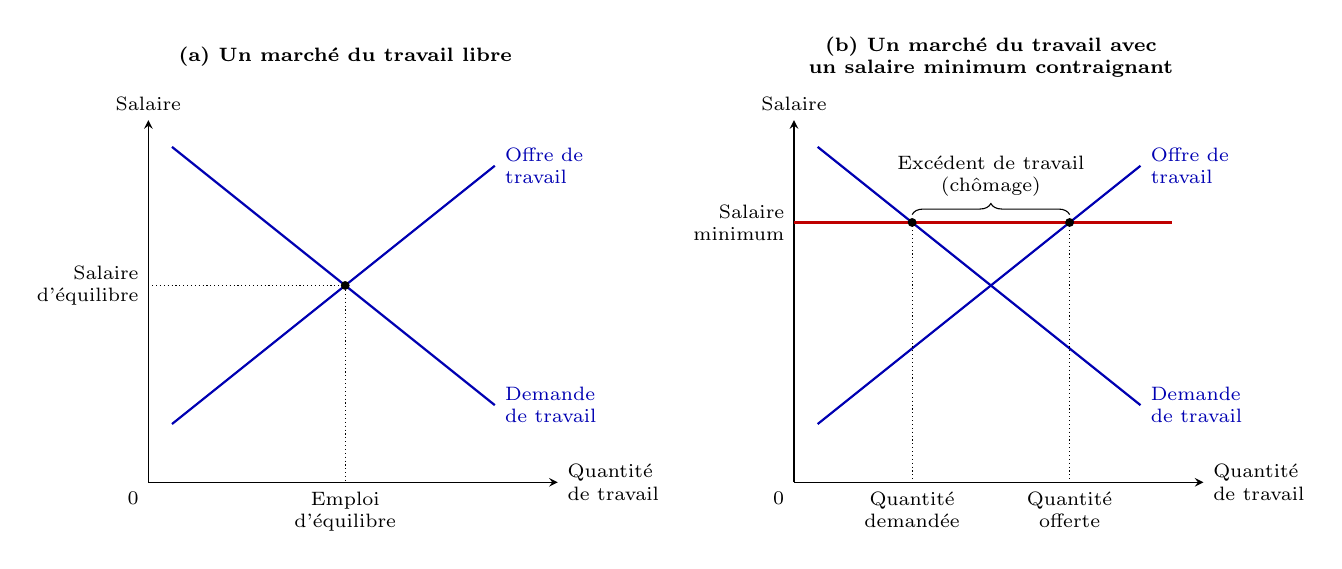
\begin{tikzpicture}[font=\scriptsize,>=stealth,
      brc/.style={decorate,decoration={brace,amplitude=4pt}}]
    % (a) un marché du travail libre
    \begin{scope}
      \node[font=\scriptsize\bfseries] at (2.5,5.4) {(a) Un marché du travail libre};
      \draw[->] (0,0) -- (5.2,0);
      \draw[->] (0,0) -- (0,4.6);
      \node[above] at (0,4.6) {Salaire};
      \node[right,align=left] at (5.2,0) {Quantité\\de travail};
      \node[below left] at (0,0) {$0$};
      \draw[blue!70!black,thick] (0.3,0.74) -- (4.4,4.02)
        node[right,align=left] {Offre de\\travail};
      \draw[blue!70!black,thick] (0.3,4.26) -- (4.4,0.98)
        node[right,align=left] {Demande\\de travail};
      \draw[densely dotted] (0,2.5) -| (2.5,0);
      \fill (2.5,2.5) circle (1.6pt);
      \node[left,align=right] at (0,2.5) {Salaire\\d'équilibre};
      \node[below,align=center] at (2.5,0) {Emploi\\d'équilibre};
    \end{scope}
    % (b) avec un salaire minimum contraignant
    \begin{scope}[xshift=8.2cm]
      \node[font=\scriptsize\bfseries,text width=6cm,align=center] at (2.5,5.4)
        {(b) Un marché du travail avec un salaire minimum contraignant};
      \draw[->] (0,0) -- (5.2,0);
      \draw[->] (0,0) -- (0,4.6);
      \node[above] at (0,4.6) {Salaire};
      \node[right,align=left] at (5.2,0) {Quantité\\de travail};
      \node[below left] at (0,0) {$0$};
      \draw[blue!70!black,thick] (0.3,0.74) -- (4.4,4.02)
        node[right,align=left] {Offre de\\travail};
      \draw[blue!70!black,thick] (0.3,4.26) -- (4.4,0.98)
        node[right,align=left] {Demande\\de travail};
      \draw[red!75!black,thick] (0,3.3) -- (4.8,3.3);
      \node[left,align=right] at (0,3.3) {Salaire\\minimum};
      \draw[densely dotted] (1.5,3.3) -- (1.5,0);
      \draw[densely dotted] (3.5,3.3) -- (3.5,0);
      \fill (1.5,3.3) circle (1.6pt);
      \fill (3.5,3.3) circle (1.6pt);
      \draw[brc] (1.5,3.4) -- (3.5,3.4)
        node[midway,above=3pt,align=center] {Excédent de travail\\(chômage)};
      \node[below,align=center] at (1.5,0) {Quantité\\demandée};
      \node[below,align=center] at (3.5,0) {Quantité\\offerte};
    \end{scope}
  \end{tikzpicture}
  \caption*{\small Le salaire minimum sur le marché du travail. In a free market (a)
  the wage balances the supply of and the demand for labour; a salaire minimum above
  that wage (b) leaves an excédent of labour, which is chômage.}
\end{figure}

\subsection{Effet des taxes}

A tax can be levied on the sellers of a good or on its buyers. Levied on the
sellers, it lifts the courbe d'offre by exactly its amount; levied on the buyers, it
pushes the courbe de demande down by exactly its amount. Whichever side it is
levied on, buyers and sellers each carry part of it.

\begin{example}[Une taxe de 0,50~\$ sur le marché des cornets]
  The ice-cream market is in equilibrium at 3~\$ and 100 cones. Levied on the
  sellers, a tax of 0,50~\$ per cone lifts the courbe d'offre from $S_1$ to $S_2$:
  90 cones are traded instead of 100, buyers now pay 3,30~\$, and sellers keep
  2,80~\$ once the tax is paid, so each side carries part of the tax. Levied on the
  buyers instead, the same tax lowers the courbe de demande from $D_1$ to $D_2$:
  again 90 cones are traded, sellers receive 2,80~\$, buyers pay 3,30~\$ with the
  tax included, and again both sides carry part of it. In this example the two
  cases give the same quantity and the same two prices.
\end{example}

\begin{figure}[h!]
  \centering
  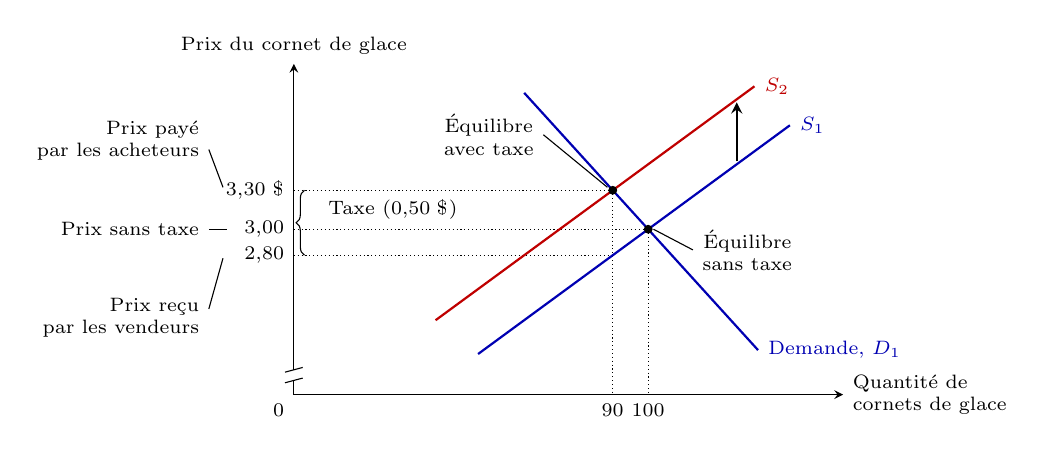
\begin{tikzpicture}[x=0.045cm,y=0.75cm,font=\scriptsize,>=stealth,
      declare function={yp(\p)=0.6+(\p-2)*2.2;},
      brc/.style={decorate,decoration={brace,amplitude=3pt}}]
    \draw[->] (0,0) -- (155,0);
    \draw (0,0) -- (0,0.24);
    \draw[->] (0,0.42) -- (0,5.6);
    \draw (-2.5,0.2) -- (2.5,0.28);
    \draw (-2.5,0.38) -- (2.5,0.46);
    \node[above] at (0,5.6) {Prix du cornet de glace};
    \node[right,align=left] at (155,0) {Quantité de\\cornets de glace};
    \node[below left] at (0,0) {$0$};
    % guides
    \draw[densely dotted] (0,{yp(3.3)}) -- (90,{yp(3.3)});
    \draw[densely dotted] (0,{yp(3)}) -- (100,{yp(3)});
    \draw[densely dotted] (0,{yp(2.8)}) -- (90,{yp(2.8)});
    \draw[densely dotted] (90,{yp(3.3)}) -- (90,0);
    \draw[densely dotted] (100,{yp(3)}) -- (100,0);
    \node[below] at (90,0) {$90$};
    \node[below] at (100,0) {$100$};
    % prices
    \node[left] at (0,{yp(3.3)}) {$3{,}30$~\$};
    \node[left] at (0,{yp(3)}) {$3{,}00$};
    \node[left] at (0,{yp(2.8)}) {$2{,}80$};
    \node[left,align=right] at (-24,4.3) {Prix payé\\par les acheteurs};
    \draw (-24,4.15) -- (-20,{yp(3.3)+0.05});
    \node[left] at (-24,{yp(3)}) {Prix sans taxe};
    \draw (-24,{yp(3)}) -- (-19,{yp(3)});
    \node[left,align=right] at (-24,1.3) {Prix reçu\\par les vendeurs};
    \draw (-24,1.45) -- (-20,{yp(2.8)-0.05});
    \draw[brc] (3,{yp(2.8)}) -- (3,{yp(3.3)});
    \node[right] at (7,{yp(3.15)}) {Taxe (0,50~\$)};
    % curves
    \draw[blue!70!black,thick] plot[domain=65:131,samples=2]
      (\x,{yp(3-0.03*(\x-100))}) node[right] {Demande, $D_1$};
    \draw[blue!70!black,thick] plot[domain=52:140,samples=2]
      (\x,{yp(3+0.02*(\x-100))}) node[right] {$S_1$};
    \draw[red!75!black,thick] plot[domain=40:130,samples=2]
      (\x,{yp(3.5+0.02*(\x-100))}) node[right] {$S_2$};
    \draw[->,thick] (125,{yp(3.5)+0.05}) -- (125,{yp(4)-0.05});
    % equilibria
    \fill (90,{yp(3.3)}) circle (1.6pt);
    \fill (100,{yp(3)}) circle (1.6pt);
    \node[align=center] (eat) at (55,4.4) {Équilibre\\avec taxe};
    \draw (eat.east) -- (88.5,{yp(3.3)+0.05});
    \node[align=center] (est) at (128,2.45) {Équilibre\\sans taxe};
    \draw (est.west) -- (101.5,{yp(3)});
  \end{tikzpicture}
  \caption*{\small Une taxe sur les vendeurs. The courbe d'offre moves up from $S_1$
  to $S_2$ by the full 0,50~\$ of the tax; at the new equilibrium, what buyers pay
  and what sellers receive are 0,50~\$ apart. The price axis is cut between 0 and
  2~\$.}
\end{figure}

\begin{figure}[h!]
  \centering
  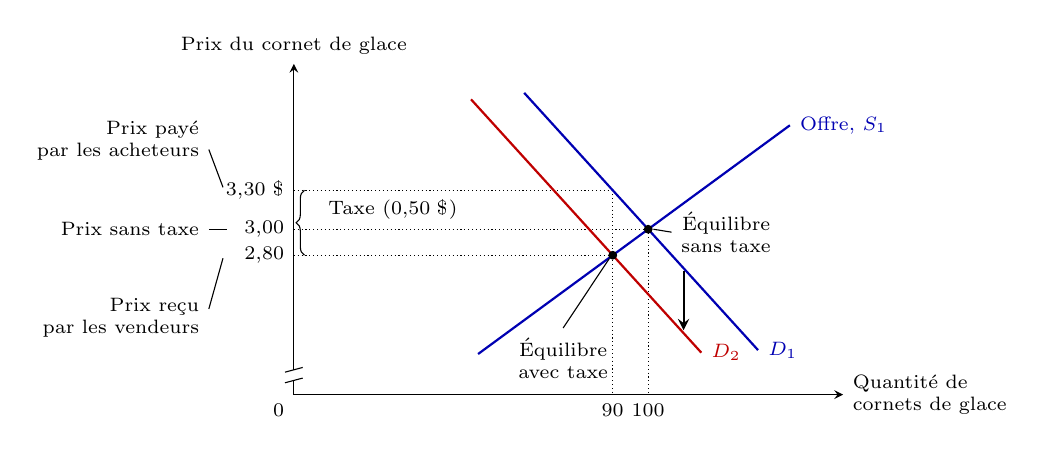
\begin{tikzpicture}[x=0.045cm,y=0.75cm,font=\scriptsize,>=stealth,
      declare function={yp(\p)=0.6+(\p-2)*2.2;},
      brc/.style={decorate,decoration={brace,amplitude=3pt}}]
    \draw[->] (0,0) -- (155,0);
    \draw (0,0) -- (0,0.24);
    \draw[->] (0,0.42) -- (0,5.6);
    \draw (-2.5,0.2) -- (2.5,0.28);
    \draw (-2.5,0.38) -- (2.5,0.46);
    \node[above] at (0,5.6) {Prix du cornet de glace};
    \node[right,align=left] at (155,0) {Quantité de\\cornets de glace};
    \node[below left] at (0,0) {$0$};
    % guides
    \draw[densely dotted] (0,{yp(3.3)}) -- (90,{yp(3.3)});
    \draw[densely dotted] (0,{yp(3)}) -- (100,{yp(3)});
    \draw[densely dotted] (0,{yp(2.8)}) -- (90,{yp(2.8)});
    \draw[densely dotted] (90,{yp(3.3)}) -- (90,0);
    \draw[densely dotted] (100,{yp(3)}) -- (100,0);
    \node[below] at (90,0) {$90$};
    \node[below] at (100,0) {$100$};
    % prices
    \node[left] at (0,{yp(3.3)}) {$3{,}30$~\$};
    \node[left] at (0,{yp(3)}) {$3{,}00$};
    \node[left] at (0,{yp(2.8)}) {$2{,}80$};
    \node[left,align=right] at (-24,4.3) {Prix payé\\par les acheteurs};
    \draw (-24,4.15) -- (-20,{yp(3.3)+0.05});
    \node[left] at (-24,{yp(3)}) {Prix sans taxe};
    \draw (-24,{yp(3)}) -- (-19,{yp(3)});
    \node[left,align=right] at (-24,1.3) {Prix reçu\\par les vendeurs};
    \draw (-24,1.45) -- (-20,{yp(2.8)-0.05});
    \draw[brc] (3,{yp(2.8)}) -- (3,{yp(3.3)});
    \node[right] at (7,{yp(3.15)}) {Taxe (0,50~\$)};
    % curves
    \draw[blue!70!black,thick] plot[domain=52:140,samples=2]
      (\x,{yp(3+0.02*(\x-100))}) node[right] {Offre, $S_1$};
    \draw[blue!70!black,thick] plot[domain=65:131,samples=2]
      (\x,{yp(3-0.03*(\x-100))}) node[right] {$D_1$};
    \draw[red!75!black,thick] plot[domain=50:115,samples=2]
      (\x,{yp(2.5-0.03*(\x-100))}) node[right] {$D_2$};
    \draw[->,thick] (110,{yp(2.7)-0.05}) -- (110,{yp(2.2)+0.05});
    % equilibria
    \fill (90,{yp(2.8)}) circle (1.6pt);
    \fill (100,{yp(3)}) circle (1.6pt);
    \node[align=center] (eat) at (76,0.62) {Équilibre\\avec taxe};
    \draw (eat.north) -- (89,{yp(2.8)-0.06});
    \node[align=center] (est) at (122,2.75) {Équilibre\\sans taxe};
    \draw (est.west) -- (101.5,{yp(3)});
  \end{tikzpicture}
  \caption*{\small Une taxe sur les acheteurs. The courbe de demande moves down from
  $D_1$ to $D_2$ by the full 0,50~\$ of the tax; the quantity traded and the two
  prices come out as with the tax on sellers. The price axis is cut between 0 and
  2~\$.}
\end{figure}

How the burden of a tax is split between buyers and sellers is the
\textbf{incidence fiscale} (\textit{tax incidence}), and it turns on the élasticité
de l'offre and the élasticité de la demande. With an élastique courbe d'offre and an
inélastique courbe de demande, panel (a), the tax drives the buyers' price up a long
way and the sellers' price down only a little, so buyers carry most of it. With an
inélastique courbe d'offre and an élastique courbe de demande, panel (b), it is the
other way round: the sellers' price drops a long way, the buyers' price hardly
moves, and sellers carry most of it. So when supply is more élastique than demand,
the incidence fiscale falls more heavily on consumers than on producers, and when
demand is more élastique than supply, more heavily on producers than on consumers.

\begin{figure}[h!]
  \centering
  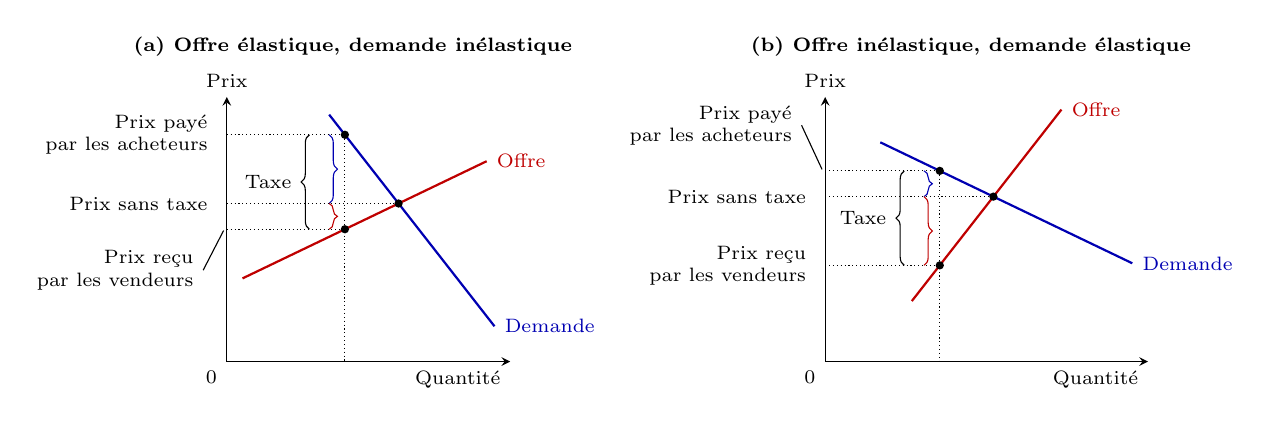
\begin{tikzpicture}[x=1.0cm,y=0.8cm,font=\scriptsize,>=stealth,
      brc/.style={decorate,decoration={brace,amplitude=3pt}}]
    % (a) offre élastique, demande inélastique
    \begin{scope}
      \node[font=\scriptsize\bfseries] at (1.6,5.0) {(a) Offre élastique, demande inélastique};
      \draw[->] (0,0) -- (3.6,0);
      \draw[->] (0,0) -- (0,4.2);
      \node[above] at (0,4.2) {Prix};
      \node[below left] at (3.6,0) {Quantité};
      \node[below left] at (0,0) {$0$};
      \draw[densely dotted] (0,3.6) -- (1.5,3.6);
      \draw[densely dotted] (0,2.509) -- (2.182,2.509);
      \draw[densely dotted] (0,2.1) -- (1.5,2.1);
      \draw[densely dotted] (1.5,3.6) -- (1.5,0);
      \draw[red!75!black,thick] (0.2,1.32) -- (3.3,3.18) node[right] {Offre};
      \draw[blue!70!black,thick] (1.3,3.92) -- (3.4,0.56) node[right] {Demande};
      \fill (1.5,3.6) circle (1.5pt);
      \fill (1.5,2.1) circle (1.5pt);
      \fill (2.182,2.509) circle (1.5pt);
      \draw[brc] (1.05,2.1) -- (1.05,3.6) node[midway,left=3pt] {Taxe};
      \draw[brc,blue!70!black] (1.3,3.6) -- (1.3,2.509);
      \draw[brc,red!75!black] (1.3,2.509) -- (1.3,2.1);
      \node[align=right,anchor=east] at (-0.12,3.6) {Prix payé\\par les acheteurs};
      \node[anchor=east] at (-0.12,2.509) {Prix sans taxe};
      \node[align=right,anchor=east] (rv) at (-0.3,1.45) {Prix reçu\\par les vendeurs};
      \draw (rv.east) -- (-0.04,2.08);
    \end{scope}
    % (b) offre inélastique, demande élastique
    \begin{scope}[xshift=7.6cm]
      \node[font=\scriptsize\bfseries] at (1.85,5.0) {(b) Offre inélastique, demande élastique};
      \draw[->] (0,0) -- (4.1,0);
      \draw[->] (0,0) -- (0,4.2);
      \node[above] at (0,4.2) {Prix};
      \node[below left] at (4.1,0) {Quantité};
      \node[below left] at (0,0) {$0$};
      \draw[densely dotted] (0,3.027) -- (1.455,3.027);
      \draw[densely dotted] (0,2.618) -- (2.136,2.618);
      \draw[densely dotted] (0,1.527) -- (1.455,1.527);
      \draw[densely dotted] (1.455,3.027) -- (1.455,0);
      \draw[red!75!black,thick] (1.1,0.96) -- (3.0,4.0) node[right] {Offre};
      \draw[blue!70!black,thick] (0.7,3.48) -- (3.9,1.56) node[right] {Demande};
      \fill (1.455,3.027) circle (1.5pt);
      \fill (1.455,1.527) circle (1.5pt);
      \fill (2.136,2.618) circle (1.5pt);
      \draw[brc] (1.005,1.527) -- (1.005,3.027) node[midway,left=3pt] {Taxe};
      \draw[brc,blue!70!black] (1.255,3.027) -- (1.255,2.618);
      \draw[brc,red!75!black] (1.255,2.618) -- (1.255,1.527);
      \node[align=right,anchor=east] (pa) at (-0.3,3.75) {Prix payé\\par les acheteurs};
      \draw (pa.east) -- (-0.04,3.05);
      \node[anchor=east] at (-0.12,2.618) {Prix sans taxe};
      \node[align=right,anchor=east] at (-0.12,1.527) {Prix reçu\\par les vendeurs};
    \end{scope}
  \end{tikzpicture}
  \caption*{\small La répartition de la charge d'une taxe. At the quantity sold with
  the tax, the tax separates the price buyers pay from the price sellers receive;
  the blue brace is the buyers' share, from the price without the tax up to the
  price they pay, and the red brace the sellers' share. The less élastique side of
  the market bears the larger share.}
\end{figure}

\subsubsection{Effet des taxes : limites}

Three limits of taxation are named, and none is developed:
\begin{itemize}
  \item Nozick / Wilt Chamberlain (star NBA des années 60 et 70)~;
  \item vote par les pieds, illustrated by a press headline: the billionaire Chris
    Rokos, a hedge-fund manager who paid £330m in tax the previous year, is leaving
    the United Kingdom, the latest financier to go as the very rich fear tax
    rises;
  \item courbe de Laffer.
\end{itemize}
